%
% ----------------------------------------------------------------
% *************************PhD Thesis ************************
% ----------------------------------------------------------------
%\documentclass[twoside,openright,a4paper,fleqn]{book}
%\usepackage{a4}
\documentclass[final,a4paper]{book}
\usepackage[T1]{fontenc}
\usepackage[ansinew]{inputenc}
\usepackage{latexsym,amssymb}
\usepackage{makeidx}
\usepackage[chapter]{tocbibind}
\renewcommand{\figurename}{\footnotesize\sc Figure\rm}
\renewcommand{\tablename}{\footnotesize\sc Table\rm}

\usepackage[active]{srcltx}
\usepackage{fancyhdr}
\usepackage{graphicx}
\usepackage{epsfig}
\usepackage{algorithm}
\usepackage{algpseudocode}
\usepackage{url}
\usepackage{mathtools}

\usepackage[italian]{babel}

%\usepackage[refpages]{gloss}

%\usepackage{subfigure} % was: subfignarms.sty
%\usepackage{psfig}


\usepackage{layout}
%Theorem
\newtheorem{theorem}{Theorem}
\newtheorem{lemma}{Lemma}
\newtheorem{definition}{Definition}
\newtheorem{notation}{Notation}

% ----------------------------------------------------------------
\vfuzz2pt % Don't report over-full v-boxes if over-edge is small
\hfuzz2pt % Don't report over-full h-boxes if over-edge is small

% ENVIRONMENTS --------------------------------------------------
\newlength{\larghezza}
\newlength{\inizio}


% ---------- intro -----------------------------------------------

\makeindex

% ---------- Glossary -------------------------------------
%\makegloss

% ---------- End Glossary ---------------------------------------

\linespread {1.3}

\oddsidemargin=54pt
\evensidemargin=54pt

\begin{document}
%\layout

\pagestyle{fancy}
\fancyhf{}
\fancyhead[RL]{\rightmark}
\fancyhead[LO]{\leftmark}
\fancyhead[LE,RO]{\small \thepage}

\renewcommand{\chaptermark}[1]{\markboth{\sc\small #1}{}}
\renewcommand{\sectionmark}[1]{\markright{\sc\small \thesection\ #1}}

%\pagenumbering{Roman}

%Titolo da rivedere e confermare
\title{\sc \LARGE Classification and Prediction on sequential data using Recurrent Neural Networks}
\author{\LARGE \textit{Luigi Clemente}\\
Dipartimento di Informatica\\
Dottorato in Informatica XXIII ciclo\\
\sc Universit\`a degli Studi di Bari ``Aldo Moro''\\
\sl Via E. Orabona, 4 - 70125 Bari, \sc Italy\\
\tt luigi.clemente@gsquare.it
}
\date{
%\begin{figure}[h]
 % \centering
  %\includegraphics[width=3cm]{fig/eu-flag.png}
%\end{figure}
\vspace{1cm}
S.S.D.: INF/01\\
\vspace{2cm}
Supervisore: Prof. Donato Malerba\\
\vspace*{\fill}
\begin{tabular}{c}
	\hline
	\it A dissertation submitted in partial fulfillment \\
	\it of the requirements for the degree of\\
	{\sc Doctor of Philosophy in Computer Science}\\
	\hline	\\
	16 Ottobre 2015
\end{tabular}
}

% ----------------------------------------------------------------

\pagenumbering{roman}

\maketitle

\clearpage

\section*{Crediti}
Questa tesi \`e stata impaginata usando i seguenti programmi open-source:
\begin{itemize}
  \item [$\circ$] TeXShop LaTeX Editor \\
	available at: {\tt http://www.uoregon.edu/$\sim$koch/texshop/}
  \item [$\circ$] MacTex Distribution \\
	available at: {\tt http://www.tug.org/mactex/}
\end{itemize}
\vspace*{\fill}


\noindent
\begin{tabular}{p{185pt} p{110pt}}
Supervisore Tesi \hskip 3cm \ & \\ \cline{2-2} & Prof. Donato Malerba \\
\end{tabular}

\vspace{2cm}

\noindent
\begin{tabular}{p{185pt} p{110pt}}
Presidente del Comitato di Supervisione \hskip 2cm \ & \\ \cline{2-2}
\end{tabular}
\vspace{1cm}

\noindent
\begin{tabular}{p{185pt} p{110pt}}
Membro  del Comitato di Supervisione \hskip 2cm \ & \\ \cline{2-2}
\end{tabular}
\vspace{1cm}

\noindent
\begin{tabular}{p{185pt} p{110pt}}
Membro  del Comitato di Supervisione  \hskip 2cm \ & \\ \cline{2-2}
\end{tabular}
\vspace{2cm}


\vspace*{\fill} \noindent \hrule
\begin{tabular}{l}
	Presentato il {\sl XXXX Date to define}\\
	Copyright {\copyright} 2015 Luigi Clemente\\
\end{tabular}
\hrule


% ----------------------------------------------------------------
% insert toc
\tableofcontents
% ----------------------------------------------------------------
% insert Lists
\listoffigures
\listoftables
% ----------------------------------------------------------------
% insert Acknowledgments

\chapter*{Riconoscimenti}
\addcontentsline{toc}{chapter}{Riconoscimenti}
\pagenumbering{arabic}
\markboth{\sc Riconoscimenti}{\sc Riconoscimenti}

\input{ack}
% ----------------------------------------------------------------
% insert Abstract
\chapter*{Sommario}
\addcontentsline{toc}{chapter}{Sommario}
\markboth{\sc Sommario}{\sc Sommario}
Innumerevoli compiti richiedono la consapevolezza del tempo. Ad esempio l'assegnare didascialia ad immagini, effettuare una sintesi vocale o giocare ad un video gioco sono tutti compiti che richiedono un modello in grado di generare delle sequenze di output. In altri ambiti, come la predizione ti time series o l'analisi video sono richiesti modelli capaci di apprendere da sequenze di input. Inoltre compiti di gran lunga pi\`u interattivi come la traduzione di testi in linguaggio naturale richiedono modelli che apprendano da sequenze di input e generino sequenze di output.


Le Reti Neurali Ricorrenti (o Recurrent Neural Networks RNNs) costituiscono un sottoinsieme di reti neurali in grado di catturare le dinamiche temporali attraverso l'uso di cicli nel grafo delle connessioni. A differenza delle reti neurali tradizionali, le reti ricorrenti possono analizzare i campioni uno alla volta mantenendo uno stato, o memoria, che riflette una finestra contestuale arbitrariamente lunga. Mentre queste reti sono state a lungo ritenute troppo difficili da addestrare dato che spesso contengono milioni di parametri, i recenti progressi nelle architetture di rete, nelle tecniche di ottimizzazione e nella computazione parallela hanno reso possibile l'apprendimento su larga scala con le RNNs.


Negli ultimi anni sistemi basati su architetture di reti ricorrenti come Long Short Term Memory (LSTM) hanno dimostrato delle performance da record in vari compiti come l'image captioning, traduzioni linguistiche e riconoscimento della scrittura.


In questa tesi utilizzeremo una LSTM per creare un Part-Of-Speech (POS) Tagger. In linguistica il pos tagging \`e un processo che assegna ad ogni parola di un testo una particolare parte del discorso (es. sostantivio, aggettivo, pronome ecc..). Questa assegnazione viene fatta basandosi sia sulla parola stessa che sul contesto. L'addestramente della rete avverr\`a a livello di carattere e non di parola. Il dataset di training, infatti, verr\`a passato alla rete un carattere alla volta. Lo scopo \`e quello di valutare le performance della rete LSTM cos\`i addestrata.

% ----------------------------------------------------------------
\clearpage
% ----------------------------------------------------------------


\chapter {Introduzione}\label{chap:chap_1}
\nocite{Lipton:2009}
Fin dagli albori dell'informatica l'uomo \`e sempre stato affascinato dalla possibilit\`a di creare un'intelligenza artificiale - macchine in grado di riprodurre la complessit\`a dei comportamenti umani.
Alan Turing, uno dei padri dell'informatica moderna, ha dimostrato come qualsiasi problema computabile pu\`o essere eseguito da una Macchina di Touring Universale~\cite{wiki:MacchinaTuring} - quindi, se la mente umana pu\`o essere descritta da un algoritmo allora una qualsiasi Macchina di Turing \`e abbastanza potente da rappresentarla.

Tutti i computer odierni sono Turing Completi, il che significa che possono rappresentare ogni tipo di algoritmo computabile.
Il problema quindi \`e trovare il giusto algoritmo capace di simulare il comportamento umano; tuttavia, questo risulta troppo complesso per essere risolto nell'immediato ma possiamo pensarea a diversi approcci - ad esempio - possiamo partire creando macchine in grado di riconoscere semplici immagini come numeri scritti, migliorarle rendendole capaci di riconoscere volti umani e proseguendo cos\`i fino alla creazione di macchine con la stessa abilit\`a umana di riconoscere oggetti nel mondo reale.

Un approccio alternativo consiste nel simulare il cervello umano a livello di neuroni.
Con la tecnologia attuale possiamo simulare la realt\`a in modo molto realistico, basti pensare ai progressi fatti in campo videoludico o cinematografico; risulta perci\`o abbastanza realistico ipotizzare che, con la giusta rappresentazione di un neurone e sufficiente capacit\`a di calcolo, sia possibile simulare un cervello umano e creare macchine intelligienti.

Ed \`e proprio da questa intuizione che nasce il concetto di reti neurali artificiali.

\section{Reti Neurali}
Gli studi sul sistmea nervoso umano hanno ispirato il concetto di rete neurale artificiale.
In una rete neurale artificiale, dei semplici nodi artificiali (detti "neuroni" o "unit\`a") sono collegati gli uni agli altri in modo da formare una rete che imitia una rete neurale biologica.

Non esiste un'unica definizione formale di cosa \`e una rete neurale.
Comunque, una classe di modelli statistici possono essere chiamati "neurali" se hanno le seguenti caratteristiche:

\begin{itemize}
  \item contengono un insieme di pesi, ad esempio dei parametri numerici che vengono regolati tramite un algoritmo di apprendimento
  \item sono capaci di approssimare una funzione non lineare degli input
\end{itemize}

Si pu\`o pensare a questi pesi come la forza con cui i singoli neuroni sono collegati gli uni con gli altri, collegamenti che vengono attivati durante le fasi di addestramento e predizione.

Nelle attuali implementazioni software delle reti neurali, l'approccio ispirato alla biologia \`e stato per lo pi\`u abbandonato in favore di un'approccio pi\`u pratico basado sulla statistica e sulla teoria dei segnali.

La prima e pi\`u semplice tipologia di rete neurale ideata \`e stata la \emph{feedforward neural network}.
In queste reti le infomrazioni viaggiano in una sola direzione, in avanti (forward) dall'input verso l'output attraversando eventuali nodi nascosti.
Le connessioni tra le unit\`a della rete non formano cicli diretti (Figura~\ref{fig:feedforwardNeuralNetwork}).

\section{Il Tempo} %TODO cambiare titolo?
Un grosso limite delle reti neurali feedforward \`e l'incapacit\`a di modellare esplicitamente il tempo.
Tutta via le reti feedforward, cos\`i come altri modelli per l'apprendimento automatizzato (es. support vector machine), si sono dimostrate estremamente capaci anche senza una modellazione esplicita del tempo.
Anzi, probabilmente \`e proprio grazie a questa assunzione di indipendenza fra i campioni di una sequenza di input che negli ultimi anni siamo stati in grado di avanzare cos\`i tanto nel campo del machine learning.
In pi\`u molti modelli cercando di catturare il tempo concatenando i singoli input o con un valore numerico, a rappresentare l'ordine temporale, o con i suoi diretti successori o predecessori nella sequenza degli input fornendo cos\`i una sorta di contesto.

Sfortunatamente, nonostante l'utilit\`a dell'assunzione di indipendenza, questa rende impossibile modellare delle dipendenze temporali a lungo raggio.
Ad esempio, un modello addestrato con una finestra contestuale di lunghezza finita pari a 5 non sar\`a mai in grado di rispondere a semplici domande del tipo ``\emph{qual \`e stata l'informazione vista 10 unit\`a temporali fa?}''.
Per applicazioni pratiche, come ad esempio l'automatizzazione di un call center, un sistema limitato come questo potrebbe riuscire ad indirizzare correttamente le chiamate ma non potrebbe mai partecipare ad una coversazione.

Fin dai primi modelli di intelligenza artificiale, abbiamo cercato di creare sistemi capaci di interagire con gli esserei umani.
Alan Turing, nel suo saggio \emph{Computing Machinery and Intelligence}, propose un ``Gioco dell'Imitazione'' con il quale giudicare l'intelligenza di una macchina in base alla sua abilit\`a di sostenere un dialogo convincente con un essere umano~\cite{Turing:1950}.
Oltre a sistemi in grado di sostenere un dialogo convincente, ne esistono molti altri la cui realizzazione sarebbe altrettanto utile ed importante (es. automobili capaci di spostarsi in autonomia e sistemi di chirurgia robotica) e sembra molto improbabile riuscire a raggiungere certi risultati senza utlizzare una modellazione esplicita del tempo.

Le \emph{reti neurali ricorrenti} (\emph{RNN}) sono state pensate proprio per superare questi limiti.
Si tratta di un sovrainsieme delle reti neurali feedforward con la capacit\`a di passare informazioni attraverso fasi temporali e, per questo, in grado di eseguire quasi ogni tipo di computazione.

Un noto risultato di Siegelman and Sontag del 1991 dimostra come una rete neurale ricorrente di dimensione finita e con delle funzioni sigmoide come funzioni di attivazione possa simulare una macchina di Turing universale~\cite{Siegelmann:1991}.
In pratica, l'abilit\`a di modellare dipendenze temporali rende le reti neurali particolarmente adatta a compiti dove i dati in input e/o output sono costutiti da sequeze di valori che sono dipendenti gli uni dagli altri (Figura~\ref{fig:simpleRecurrentNeuralNetwork}).

\section{Modelli di Markov} %TODO pensare ad un titolo piu' appropiato
Le reti neurali ricorrenti per\`o non sono stati i primi modelli a catturare le dipendenze temporali.
Le \emph{catene di Markov}, che modellano le transizioni tra sequenze di stati $(s^{(1)}, s^{(2)}, \dots, s^{(T)},)$, sono state inizialmente descritte dal matematico Andrey Markov nel 1906.
I \emph{modelli di Markov nascosti} (\emph{HMM}), che modellano i dati osservati $(o^{(1)}, o^{(2)}, \dots, o^{(T)},)$ come probabilisticamente dipendenti da stati non osservati, sono stati descritti nel 1950 e sono stati largamente studiati fino agli anni '60.
In ogni caso, l'approccio tradizionale con il modello di Markov \`e piuttosto limitato perch\`e i possibili stati possono essere presi solo da un piccolo spazio discreto di stati $ s_j \in S$.
L'algoritmo Viterbi, usato in fase di apprendimento, ha una complessit\`a in tempo pari ad $O(|S|^2)$.
In pi\`u la matrice di transizione, che cattura la probabilit\`a di muoversi da uno stato in uno dei possibili stati adiacenti, ha dimensione $|S|^2$.
Quindi, risulta impossibile utilizzare un HMM quando l'insieme dei possibili stati nascosti \`e pi\`u grande di circa 106.
Inoltre, ciascun stato nascosto $s^{(t)}$ pu\`o dipendere solo dallo stato precedente $s^{(t+1)}$
E nonostante sia possibile estendere il modello di Markov in modo da gestire pi\`u di un solo stato precedente aumentando cos\`i la finestra contestuale usata per l'apprendimento, questo porterebbe anche ad una crescita esponenziale dello spazio degli stati, rendendo il modello di Markov computazionalmente impraticabile per modelli con dipendenze a lungo raggio.

Queste limitazioni invece non si pongono per le reti neurali ricorrenti.
Le reti neurali ricorrenti, infatti, possono catturare dipendenze temporali a lungo raggio, superando le limitazioni imposte dal modello di Markov.
Cos\`i come nei modelli di Markov, ogni stato in una RNN tradizionale dipende solo dai valori di input correnti e dallo stato della rete nella precedente fase temporale\footnote{Le \emph{reti neurali ricorrenti bidirezionali} (\emph{BRNN})~\cite{Schuster:1997} estendono le RNN per modellare dipendenze con osservazioni passate e future mentre le tradizionali RNN modellano dipendenze solo con osservazioni passate.}.
Tuttavia, gli stati nascosti possono contenere, ad ogni fase temporale, informazioni provenienta da una finestra contestuale arbitrariamente lunga.
Questo \`e possibile grazie al fatto che il numero di stati distinti che possono essere rappresentati da un livello nascosto di nodi cresce in maniera esponenziale all'aumentare del numero dei nodi presenti nel livello.
Anche se ciascun nodo pu\`o rappresentare solo valor binari, un singolo livello nascosto pu\`o rappresentare $2^N$ stati distinti dove $n$ \`e il numero di nodi presenti.
Con dei valori reali invece, anche tenendo conto del limite imposta dalla rappresentazione a 64 bit dei numeri, un singolo livello nascosto pu\`o rappresentare $2^64N$ stati distinti.
Nonostante il potenziale potere espressivo della rete cresce in maniera esponenziale, la complessit\`a di addestramento e predizione cresce in ordine quadratico.

\mytodo{aggiungere altro?} %TODO aggiungere altro?


\chapter {Stato dell'arte}\label{chap:chap_2}
In questo capitolo introduciamo notazioni formali e diamo una breve spiegazione del funzionamento delle reti neurali e degli strumenti utilizzati.

\section{Il Tempo}

Le RNN non sono limitate a sequenze indicizzate in maniera temporale.
Sono state usate con successo anche per seqenze di dati non temporali, come ad esempio i dati genetici.
In ongi caso, la computazione procede nel tempo e molte importanti applicazioni hanno un aspetto temporale esplicito o implicito.

Nonostante, in questa tesi, ci riferiremo al tempo i metodi descritti sono applicabili ad una famiglia pi\`u ampia di compiti.
Parlando di tempo ci riferiamo ad un campione $x^{(t)}$ in input e ad un valore atteso $y^{(t)}$ in output che sono generati in \emph{sequenze di fasi temporali} discrete indicate da $t$
La nostra sequenza pu\`o essere formata da un numero finito di campioni o da un numero infinito ma numerabile di campioni.
Se abbiamo a che fare con un numero finito di campioni allora possiamo indicare con $T$ il massimo indice temporale.
Quindi una sequenza di valori di input consecutivi pu\`o essere scritta come $(x^{(1)}, x^{(2)}, \dots, x^{(T)})$ mentre gli output come $(y^{(1)}, y^{(2)}, \dots, y^{(T)})$.
Questi valori possono essere dei campioni, presi ad intervalli regolari di tempo, di un processo reale continuo come ad esempio i fotogrammi che compongono un video.
Gli intervalli di tempo possono anche essere dei semplici valori ordinali senza una durata esatta.
\`E il caso, ad esempio, delle sequenze genetiche che hanno un ordine ma non un ordine temporale o ancora del linguaggio naturale dove le parole hanno un ordine logico ben preciso che, tuttavia, non corrisponde ad intervalli di temporali ben defniti.
Ad esempio nella frase ``\emph{Lisa suona il sassofono}'' abbiamo che $x^{(1)}$ = Lisa, $x^{(2)}$ = suona, ecc. Ciascuna parola corrisponde ad intervalli di tempo che non sono costanti, ``\emph{il}'' e ``\emph{sassofono}'' hanno bisogno di tempi diversi per essere pronunciati.

\section{Reti Neurali}
Le reti neurali sono modelli computazionali ispirati dalla biologia del sistema nervoso centrale.
Generalmente una rete neurale \`e formata da un insieme di \emph{neuroni artificiali}, comunemente chiamati \emph{nodi} o \emph{unit\`a}, collegati da un insieme di archi diretti che, intuitivamente, rappresentano le \emph{sinapsi} di una rete neurale biologica.
Associato ad ogni neurone $j$ vi \`e una funzione di attivazione $l_j$, chiamata anche funzione di collegamento (o funzione link).
In questa tesi user\`o la notazione ``$l_j$'' invece di ``$h_j$'' (notazione usata in altri documenti) per distinguere la funzione di attivazione $l_j$ dal valore dei nodi nascosti in una rete, che vengono comunemente indicati con \textbf{h} nella letteratura delle RNN.

Associato ad ogni arco dal nodo $j^{'}$ al nodo $j$ vi \`e un peso $w_{jj^{'}}$. Seguento la convenzione adottata in molti altri documenti che trattano reti neurali, indicheremo i neuroni con $j$ e $j^{'}$ mentre, con $w_{jj^{'}}$, indicheremo il peso corrispondente all'arco diretto che parte dal nodo $j^{'}$ e arriva al nodo $j$.
\`E importante notare che in altri documenti e libri, come ad esempio su Wikipedia, gli indici dei pesi sono invertiti e che $w_{j^{'}j} \neq w_{jj^{'}}$ indica il peso sull'arco diretto dal nodo $j^{'}$ al nodo $j$.

Il valore $v_j$ di ciascun neurone $j$ \`e calcolato applicando la sua funzione di attivazione ad una somma pesata dei suoi valori di input (\mytodo{Aggiungere un'immagine!}): %TODO pensare ad un titolo piu' appropiato
\begin{equation} % \begin{equantion*} per non numerare l'equazione
  v_j = l_j\left( \sum_{j^{'}} w_{jj^{'}} \cdot v_{j^{'}} \right)
\end{equation}
Per comodit\`a, ci riferiremo alla somma pesata all'interno delle parentesi come l'\emph{attivazione in arrivo} e la indicheremo con $a_j$. Rappresentiamo l'intero processo in figura disegnando i neuromi coe dei cerchi mentre gli archi come delle frecce che li collegano.
Quando possibile, verr\`a utilizato un simbolo per indicare l'esatta funzione di attivazione utilizzata, ad esempio $\sigma$ per la fnzione sigmoide.

Scelte abbastanza comuni per la funzione di attivazione includono la funzione sigmoide $\sigma(z) = 1/(1+e^{-z})$ e la funzione \emph(tanh) $\phi(z)=(e^z-e^{-z})/(e^z+e^{-z})$ che \`e diventata molto comune nelle reti neurali di tipo \emph{feedforward} ma \`e stata utilizzata anche in reti neurali ricorrenti~\cite{Sutskever:2011}.
Un'altra funzione di attivazione che \`e diventata lo stato dell'arte nella ricerca di deep learning \`e la funzione ReLU (\emph{rectified linear unit}) $l_j(z)=\operatorname{max}(0, z)$.
Questa funzione ha dimostrato di poter migliorare le prestazioni di molte reti neurali in una grande variet\`a di applicazioni, che spaziano dal riconoscimento vocale al riconoscimento di oggetti, ed \`e stata utilizzata anche in reti neurali ricorrenti~\cite{Bengio:2013}.

La funzione di attivazione da applicare sui nodi di output dipende dall'applicazione.
Per una classificazione a pi\`u classi, applichiamo al livello di output una funzione non lineare softmax.
La funzione softmax calcola l'output come:
\begin{equation}
  \hat{y_k} = \frac{e^{a_k}}{\sum_{k^{'}=1}^{K} e^{a_{k^{'}}}}
\end{equation}
dove $K$ \`e il numero totale di possibili output (classi). Il denominatore \`e una funzione di normalizzazione che consiste nella somma di funzioni esponenziali dei valori dati in output da tutti i nodi e serve per assicrarsi che l'output totale sommi ad 1.
Nel caso di regressioni invece viene comunemente utilizzata una funzione lineare come output.
Dato che nella maggioranza dei casi le reti neurali, specialmente quelle ricorrenti, vengono utilizzate per applicazioni che coinvolgono la classificazione, durante questa tesi, a meno che diversamente specificato, daremo per scontato l'uso della funzioen softmax come output.

\section{Reti Neurali Feedforward}
Con un modello computazionale a rete neurali, \`e necessario determinare l'ordine con cui la computazione dovrebbe procedere.
I nodi dovrebbero essere calcolati uno alla volta e poi aggiornati, oppure i valori di tutti i nodi dovrebbero essere calcolati iniseme per poi applicare tutti gli aggiornamenti simultaneamente?
Le \emph{reti neurali feedforward} (\mytodo{aggiungere figura ffnn}) sono una classe ristretta di reti neurali che affrontano questo prolema proibnedo i cicli dal grafo delle connessioni neurali. %TODO aggiungere immagine
In questo modo tutti i nodi possono essere disposti in livelli.
I valori in output di ciascun livello possono essere calcolati solo a partire dai valori di output dei livelli precedenti.

L'input $x$ viene dato in pasto ad una rete neurale feedforward impostando i valori dei nodi del livello pi\`u in basso.
I valori dei nodi di ciascuno dei livelli superiori non potranno essere calcolati finch\`e non saranno disponibili i valori in output $\hat{y}$ dei livelli inferiori.
Queste tipologie di reti sono usate di frequente per applicazioni di apprendimento supervisionato come classificazione e regressione.
L'apprendimento \`e ottenuto aggiornando iterativamente i pesi dei singoli archi in modo da minimizzare una funzione di perdita, $\mathcal{L}(\hat{y},y)$, che penalizza la distanza fra l'output desiderato $y$ e l'output predetto $\hat{y}$ tramite tecniche di ottimizzazione.
Nonostante l'algoritmo di ottimizzazione esatto \`e un noto problema NP-Completo, una grande quantit\`a di euristiche pre addestramento e avanzate tecniche di ottimizzazione hanno condotto ad un impressionante numero di successi empirici su molte applicazioni di apprendimento supervisionato.

L'algoritmo utilizzato con maggiore successo per addestrare una rete neurale \`e l'algoritmo di backpropagation, introdotto da Rumelhart et al. nel 1985~\cite{Rumelhart:1985}.
Questo algoritmo usa la regola della catena per calcolare la derivata di una funzione di perdita $\mathcal{L}$ rispetto ciascun parametro nella rete.
I pesi sui singoli archi vengono poi tramite la discesa dei gradienti.
Dato che la superficie di perdita non \`e convessa non vi \`e alcuna garanzia che l'algoritmo di backpropagation riesca a trovare un minimo globale.
Ci\`o nonostante, nella pratica, reti addestrate in questo modo hanno ottenuto notevoli successi.

Tuttavia le reti feedforward sono limitate.
Dopo che ciascun campione \`e stato processato l'intero stato della rete viene perso.
Se i campioni sono indipendenti gli uni dagli altri questo non presenta assolutamente un problema.
Ma se i dati sono in una relazione temporale, questo non \`e accettabile.
I fotogrammi di un video o le parole di una frase rappresentano situazioni in cui l'assunzione di indipendenza fallisce.

\section{Reti Neurali Ricorrenti}
Le \emph{reti neurali ricorrenti} costituiscono un sovrainsieme proprio delle reti neurali feedforward che, a differenza di quest'ultime, includono degli archi ricorrenti.
Questi archi ricorrenti si estendono su intervalli temporali adiacenti e introducono il concetto di tempo nel modello.
Mentre le RNN possono non contenere cicli tra gli archi convenzionali, gli archi ricorrenti possono formare cicli.
Al tempo $t$, i nodi che ricevono un input da un arco ricorrente, ricevono un \emph{input di attivazione} sia dal campione corrente $x^({t})$ che dai nodi nascosti $h^{(t-1)}$ del precedente stato della rete.
L'output $\hat(y^{(t)})$ \`e poi calcolato in base allo stato nascosto $h^{(t)}$ del tempo $t$.
Quindi, l'input $x^({t})$ al tempo $t-1$ pu\`o influenzare l'output $\hat(y^{(t)})$ al tempo $t$ proprio grazie a queste connessioni ricorrenti.

Le seguenti due equazioni, mostrano i calcoli necessari per eseguire, per ogni fase temporale, il passaggio in avanti dei dati di una semplice rete neurale ricorrente:
\begin{equation}
  h^{(t)} = \sigma(W_{hx}x + W_{hh}h^{(t-1)} + b_h)
\end{equation}
\begin{equation}
  \hat{y}^{(t)} = \operatorname{softmax}(W_{yh}h^{(t)} + b_y)
\end{equation}

dove $W_{hx}$ \`e la matrice dei pesi tra il livello di input e il livelo nascosto mentre $W_{hh}$ \`e la matrice dei pesi ricorrenti fra i livelli nascosti di due fasi temporali adiacenti.
I vettori $b_h$ e $b_y$ rappresentano uno scostamento (\emph{bias}) che permettono a ciascun nodo di apprendere un offset.

I modelli discussi in questa tesi consistono in reti con livelli nascosti ricorrenti.
Tuttavia, sono stati proposti modelli, come la rete di Jordan, che ammettono la presenza di connessioni tra gli output della rete in uno stato e il livello nascosto della rete nello stato successivo.

Una semplice rete neurale \`e mostrata in \mytodo{aggiungere immagine rnn}. %TODO aggiungere immagine
La dinamica di questa rete attravesso pi\`u fasi temporali pu\`o essere visualizzata \emph{dispiegando} la rete (\mytodo{aggiungere immagine}). %TODO aggiungere immagine
Con questa visualizzazione, il modello pu\`o essere interpretata come una rete non ciclica, ma piuttosto come una rete con un livello per intervallo di tempo a dei pesi condivisi tra gli intervalli temporali.
Diventa quindi chiaro come una rete dispiegata in questo modo pu\`o essere addestrata attraverso pi\`u fasi temporali usando l'algoritmo di backpropagation.
Questo algoritmo viene chiamato \emph{backpropagation through time} (BPTT, backpropagation attraverso il tempo), ed \`e stata introdotta nel 1990~\cite{Werbos:1990}

\subsection{Addestramento}
L'apprendimento con le reti neurali ricorrenti \`e stato a lungo visto come qualcosa di difficile.
Cos\`i come per tutte le reti neurali, l'ottimizzazione della funzione di perdita \`e un problema NP-Completo.
Ma l'apprendimento con le reti ricorrenti pu\`o essere reso ancora pi\`u complesso a causa della difficolt\`a nell'apprendere delle dipendenze a lungo raggio.
Il noto problema della \emph{scomparsa} ed \emph{esplosione} dei gradienti si verifica quando l'errore viene propagato attraverso molte fasi temporali.
\mytodo{dire di pi\`u a riguardo?} L'impatto dell'input al tempo $\mathcal{T}$ sull'output al tempo $t$ esploder\`a esponenzialmente oppure raggiunger\`a rapidamente zero al crescere di $\mathcal{T} - t$, a seconda se il peso $\abs{w_{jj}}>1$ oppure $\abs{w_{jj}}<1$ ma anche in base alla funzione di attivazione utilizzata %TODO dire di piu
(ad esempio con una funzione di attivazione $l_j = \sigma$ si verificher\`a maggiormente il problema della sparizione del gradeinte, viceversa con la funzione ReLU $\operatorname{max}(0, x)$ il gradiente esploder\`a).

Una possibile soluzione al problema consiste nell'usare una versione leggermente modificate dell'algoritmo BPTT che prende il nome di \emph{truncated backpropagation through time} (TBPTT)~\cite{Williams:1989}.
Con l'algoritmo TBPTT viene impostato un valore che indicia il numero massimo di temporali lungo le quali pu\`o essere propagato l'errore.
In questo modo si attenua il problema dell'esplosione del gradiente perdendo, tuttavia, la capacit\`a di apprendere dipendenze a lungo raggio.

Il problema dell'ottimizzazione rappresenta un fondamentale ostacolo che non pu\`o essere risolto semplicemente modificando l'architettura della rete.
\`E noto dal 1993 che ottimizzare una rete neurale di anche solo 3 livelli costituisce un problema NP-Completo.
Tuttavia, recenti studi sia teorici che empirici, suggeriscono che il problema non \`e cos\`i insormontabile nella pratica come si potrebbe pensare.

Inoltre implementazioni sempre pi\`u performanti ed migliorate euristiche per il calcolo dei gradienti hanno reso l'addestramento delle RNN fattibile.
Ad esempio, implementazioni degli algorotmi di forward a backward propagation che sfruttano la GPU, come Theano e Torch (strumento utilizzato per gli esperimenti di questa tesi), hanno semplificato la realizzazione di veloci algoritmi di apprendimento.


\chapter {Esperimenti}\label{chap:chap_3}
In questo capitolo parler\`o dei dataset utilizzati e di come \`e stato impostato l'esperimento.

\section{Part-of-Speech (PoS) tagging}
In linguistica, il PoS tagging, \`e un processo che consisite nel raggruppare le parole di una frase in calssi dette, appunto, \emph{Part of Speech} o \emph{classi morfologiche}.
Questo raggruppamento, viene fatto sia in base alla definizione della parola stessa che al contesto in cui si trova.

Nella grammatica tradizionale, esistono un numero limitato di classi morfologiche (sostantivo, verbo, aggettivo, articolo, pronome, avverbo, congiunzione, preposizione, ecc..).

Ad esempio, possiamo classificare la frase \emph{Il cane abbaia.} in questo modo:

\centerline{Il\textbf{/ART} cane\textbf{/SOST} abbaia\textbf{/V} .\textbf{/PUNT}}

Tuttavia, chiaramente, esistono molte pi\`u classi di queste.
Per il pronome, possiamo trattare le forme singolari, plurali e possessive come classi distinte.
In molti linguaggi, inoltre, le parole possono essere distinte in base al loro ``caso'' o in base al genere.

Un esempio di classificazione pi\`u dettagliata pu\`o essere:

\begin{center}
Il\textbf{/ART:m:s}

cane\textbf{/SOST:m:s}

abbaia\textbf{/V:ind:pr:3:s}

.\textbf{/PUNT:sent}
\end{center}

In linguistica sono previste classi morfologiche per vari livelli di dettaglio, in base al modello di classificazione scelto.

Solitamente, in sistemi di PoS tagging computerizzati, vengono adottati modelli di classificazione che prevedono un numero elevato di classi (da 50 o pi\`u) e variano in base alla lingua adottata.
Esistono vari modelli comunemente accettati, quelli utilizzati per gli esperimenti di questa tesi sono:
\begin{itemize}
  \item Penn Treebank Tagset, composto da 42 classi e usato per la lingua inglese.
  \item Tanll Tagset, che conta fino a 328 classi ed \`e usato per la lingua italiana.
\end{itemize}

\section{Dataset utilizzati}
\nocite{Zanchetta:2005}
\nocite{Attardi:2008}

\subsection{CoNLL 2000}
CoNLL (\emph{Conference on Natural Language Learning}), \`e una conferenza organizzata annualmente dal gruppo \emph{SIGNLL}, a partire dal 1999.
Per ogni edizione della conferenza, sono state proposte delle attivit\`a condivise, ciascuna delle quali comprendeva dati di test e di training forniti direttamente dagli organizzatori.
In questo modo i partecipanti potevano essere valutati e confrontati in maniera sistematica.

Per gli esperimenti di questa tesi, sono stati usati i dataset di training e test forniti durante la quarta edizione della conferenza, tenutasi nel 2000.
I dati forniti consistono in file di testo contenenti, complessivamente, $253\,906$ parole che formano $10\,729$ frasi, ogni riga di ciascun file di testo corrisponde ad una parola, mentre una riga vuota denota la fine di una frase.
Ciascuna riga \`e costituita, a sua volta, da 3 colonne:
\begin{itemize}
  \item la prima colonna contiene la parola corrente
  \item la seconda colonna la classe morfologica della parola
  \item la terza riga contiene un tag che indica la parte della frase a cui, la parola corrente, appartiene
\end{itemize}

Di seguito un esempio:

\begin{center}
  \begin{minipage}{5cm}
    \begin{verbatim}
     He        PRP  B-NP
     reckons   VBZ  B-VP
     the       DT   B-NP
     current   JJ   I-NP
     account   NN   I-NP
     deficit   NN   I-NP
     will      MD   B-VP
     narrow    VB   I-VP
     to        TO   B-PP
     only      RB   B-NP
     #         #    I-NP
     1.8       CD   I-NP
     billion   CD   I-NP
     in        IN   B-PP
     September NNP  B-NP
     .         .    O
    \end{verbatim}
  \end{minipage}
\end{center}

Di seguito la lista completa di classi del modello PennTreebank (Tabell~\ref{tab:penn-tagset}):

\begin{longtable}{| c | p{.40\textwidth} | p{.50\textwidth} |} \hline
  \thead{Tag} & \thead{Descrizione} & \thead{Esempio} \\ \hline
  CC & conjunction, coordinating & and, or, but \\ \hline
  CD & cardinal number & five, three, 13\% \\ \hline
  DT & determiner & the, a, these  \\ \hline
  EX & existential there & there were six boys  \\ \hline
  FW & foreign word & mais  \\ \hline
  IN & conjunction, subordinating or preposition & of, on, before, unless  \\ \hline
  JJ & adjective & nice, easy \\ \hline
  JJR & adjective, comparative & nicer, easier \\ \hline
  JJS & adjective, superlative & nicest, easiest  \\ \hline
  LS & list item marker &   \\ \hline
  MD & verb, modal auxillary & may, should  \\ \hline
  NN & noun, singular or mass & tiger, chair, laughter  \\ \hline
  NNS & noun, plural & tigers, chairs, insects  \\ \hline
  NNP & noun, proper singular & Germany, God, Alice  \\ \hline
  NNPS & noun, proper plural & we met two Christmases ago  \\ \hline
  PDT & predeterminer & both his children  \\ \hline
  POS & possessive ending & 's \\ \hline
  PRP & pronoun, personal & me, you, it  \\ \hline
  PRP\$ & pronoun, possessive & my, your, our  \\ \hline
  RB & adverb & extremely, loudly, hard   \\ \hline
  RBR & adverb, comparative & better  \\ \hline
  RBS & adverb, superlative & best  \\ \hline
  RP & adverb, particle & about, off, up  \\ \hline
  SYM & symbol & \%  \\ \hline
  TO & infinitival to & what to do?  \\ \hline
  UH & interjection & oh, oops, gosh  \\ \hline
  VB & verb, base form & think  \\ \hline
  VBZ & verb, 3rd person singular present & she thinks  \\ \hline
  VBP & verb, non-3rd person singular present & I think  \\ \hline
  VBD & verb, past tense & they thought  \\ \hline
  VBN & verb, past participle & a sunken ship  \\ \hline
  VBG & verb, gerund or present participle & thinking is fun  \\ \hline
  WDT & wh-determiner & which, whatever, whichever  \\ \hline
  WP & wh-pronoun, personal & what, who, whom  \\ \hline
  WP\$ & wh-pronoun, possessive & whose, whosever  \\ \hline
  WRB & wh-adverb & where, when  \\ \hline
  . & punctuation mark, sentence closer & .;?*  \\ \hline
  , & punctuation mark, comma & ,  \\ \hline
  : & punctuation mark, colon & :  \\ \hline
  ( & contextual separator, left paren & (  \\ \hline
  ) & contextual separator, right paren & ) \\ \hline
  \caption{Tagset Penn Treebank} \label{tab:penn-tagset}
\end{longtable}

\subsection{Evalita 2009}
\emph{Evalita} nasce grazie all'iniziativa dell'\emph{Italian Association for Computational Linguistics} (ALIC),
ed \`e stato approvato dall'\emph{Italian Association for Artificial Intelligence} (AI*IA)
e dall'\emph{Italian Association for Speech Science} (AISV).
Lo scopo del progetto \`e quello di promuovere lo sviluppo di tecnologie in ambito linguistico,
scritto e parlato, per la lingua italiana, fornendo un ambiente condiviso nel quale
differenti sistemi e approcci, possono essere sviluppati e valutati in maniera consistente.

La diffusione di attivit\`a e di metodologie di valutazione condivise costituisce un passo fondamentale
verso lo sviluppo di risorse e tecnologie di Natural Language Processing. Il buon riscontro
ottenuto da Evalita, sia in termini di partecipanti che in termini di qualit\`a dei risultati ottenuti,
ha dimostranto che vale la pena perseguire tali obiettivi anche per la lingua italiana.
Inoltre, i dati di test e di training per le attivit\`a proposte, vengono resi disponibili alla
comunit\`a scientifica come punto di riferimenti per futuri miglioramenti.

In particolare, per questa tesi, si far\`a riferimenti all'attivit\`a di
PoS-Tagging proposta da Evalita nel 2009.

I dataset forniti dagli organizzatori sono costituiti da articoli tratti dall'edizione
online del giornale \emph{La Repubblica} (http://www.repubblica.it).

L'intero corpus \`e formato da $108\,874$ parole divise in $3\,719$ frasi.

Questo \`e stato annotato in pi\`u passaggi: il primo \`e stato portato a termina dal
gruppo di Andrea Baroni, dell'Universit\`a di Bologna, che ha classificato manualmente
l'intero corpus adottando un modello di classificazione con poche classi; successivamente
\`e stato utilizzato \emph{MorphIt!}, uno strumento automatizzato, per assegnare una lista di
possibili classi morfologiche a ciascuna parola; il risultato \`e stato poi convertito, per mezzo
di uno script, nel modello di classificazione \emph{Tanl}.

Infine, l'intero corpus \`e stato revisionato manualmente.

\subsubsection{Formato dei dati}
Il dataset di training \`e formato da un unico file di testo, con codifica UTF-8,
dove ogni riga costituisce un token seguito dalla sua classe, separati da una tabulazione,
secondo il seguente schema:

\begin{center}
  \begin{minipage}{5cm}
    \begin{verbatim}
    <TOKEN_1> <TAG1>
    <TOKEN_2> <TAG2>
    ...
    <TOKEN_N> <TAGN>
    <RIGA VUOTA>
    \end{verbatim}
  \end{minipage}
\end{center}

Al termine di ogni frase \`e presenta una riga vuota. Ad esempio:

\begin{center}
  \begin{minipage}{5cm}
    \begin{verbatim}
      A             E
      ben           B
      pensarci      Vfc
      ,             FF
      l'            RDns
      intervista    Sfs
      dell'         EAns
      on.           SA
      Formica       SP
      e'            VAip3s
      stata         VApsfs
      accolta       Vpsfs
      in            E
      genere        Sms
      con           E
      disinteresse  Sms
      .             FS

    \end{verbatim}
  \end{minipage}
\end{center}

Nell'esempio precedente vengono mostrati alcuni fra i pi\`u comuni problemi di tokenizzazione:
\begin{itemize}
  \item Le abbreviazioni vengono trattate come token (\emph{on.})
  \item Possibili espressioni multi parola non vengono trattate come un unico token (\emph{in\_genere})
  \item I clitici non vengono separati dal token (\emph{pensarci})
\end{itemize}

\subsubsection{Il modello di classificazione Tanl}
Il modello \emph{Tanl} in base alle linee guida di \emph{EAGLES}, uno standard
comunemente accettato dalla comunit\`a NLP, ed \`e derivato dalla classificazione
morfologica adottata dal corpus ISST.

Tanl \`e composto da tre livelli di classi morfologiche, ciascun livello aggiunge maggior
dettaglio alla classificazione.

Il primo livello \`e composto da 14 classi (Tabella~\ref{tab:tanl-coarse}):

\begin{table}[H]
  \centering
  \begin{tabular}{| c || l |}
    \hline
    \thead{Tag} & \thead{Descrizione} \\
    \hline
    A & adjective \\
    B & adverb \\
    C & conjunction \\
    D & determiner \\
    E & preposition \\
    F & punctuation \\
    I & interjection \\
    N & numeral \\
    P & pronoun \\
    R & article \\
    S & noun \\
    T & predeterminer \\
    V & verb \\
    X & residual class \\ \hline
  \end{tabular}
  \caption{Tagset Tanl, primo livello} \label{tab:tanl-coarse}
\end{table}

Il secondo livello del modello Tanl contiene 36 classi, di seguito riportate, con relativi esempi (Tabella~\ref{tab:tanl-fine}):
\begin{longtable}{| c | p{.20\textwidth} | p{.30\textwidth} | p{.40\textwidth} |} \hline
  \thead{Tag} & \thead{Descrizione} & \thead{Esempio} & \thead{Contesto} \\ \hline
  A & adjective & bello, buono, pauroso, ottimo  & \parbox[t]{.40\textwidth}{una \emph{bella} passeggiata\\un \emph{ottimo} attaccante\\una persona \emph{paurosa}}\\ \hline
  AP & possessive adjective & mio, tuo, nostro, loro & \parbox[t]{.40\textwidth}{a \emph{mio} parere\\il \emph{tuo} libro}\\ \hline
  B & adverb & bene, fortemente, malissimo, & \parbox[t]{.40\textwidth}{arrivo \emph{domani}\\sto \emph{bene}}\\ \hline
  BN  & negation adverb & non & \emph{non} sto bene\\ \hline
  CC & coordinative conjunction & e, o, ma & \parbox[t]{.40\textwidth}{i libri \emph{e} i quaderni\\vengo \emph{ma} non rimango}\\ \hline
  CS & subordinative conjunction & mentre, quando & \parbox[t]{.40\textwidth}{\emph{quando} ho finito vengo\\\emph{mentre} scrivevo ho finito l'inchiostro}\\ \hline
  DD  & demonstrative determiner & questo, codesto, quello & \parbox[t]{.40\textwidth}{\emph{questo} denaro\\\emph{quella} famiglia}\\ \hline
  DE & exclamative determiner & che, quale, quanto & \parbox[t]{.40\textwidth}{\emph{che} disastro!\\\emph{quale} catastrofe!}\\ \hline
  DI & indefinite determiner & alcuno, certo, tale, parecchio, qualsiasi & \parbox[t]{.40\textwidth}{\emph{alcune} telefonate\\\emph{parecchi} giornali\\\emph{qualsiasi} persona}\\ \hline
  DQ & interrogative determiner & cui, quale & i \emph{cui} libri\\ \hline
  DR & relative determiner & che, quale, quanto & \parbox[t]{.40\textwidth}{\emph{che} cosa\\\emph{quanta} strada\\\emph{quale} formazione}\\ \hline
  E & preposition & di, a, da, in, su, attraverso, verso, prima\_di & \parbox[t]{.40\textwidth}{\emph{a} casa\\\emph{prima\_di} giorno\\\emph{verso} sera}\\ \hline
  EA & articulated preposition & alla, del, nei & \emph{nel} posto\\ \hline
  FB & balanced punctuation & ( ) [ ] { } - \_ ` & \emph{(}sempre\emph{)}\\ \hline
  FF & comma, hyphen & , - & carta, penna, 30\emph{-}40 persone\\ \hline
  FS & sentence boundary punctuation & . ? ! ... & cosa\emph{?}\\ \hline
  I & interjection & ahim\`e, beh, ecco, grazie & \emph{Beh}, che vuoi?\\ \hline
  N & cardinal number & uno, due, cento, mille, 28, 2000 & \parbox[t]{.40\textwidth}{\emph{due} partite\\\emph{28} anni}\\ \hline
  NO & ordinal number & primo, secondo, centesimo & \emph{secondo} posto\\ \hline
  PC & clitic pronoun &mi, ti, ci, si, te, ne, lo, la, gli & \parbox[t]{.40\textwidth}{me \emph{ne} vado\\\emph{si} sono rotti\\\emph{mi} lavo\\\emph{gli} parlo}\\ \hline
  PD & demonstrative pronoun & questo, quello, costui, ci\`o & \parbox[t]{.40\textwidth}{\emph{quello} di Roma\\\emph{costui} uccide}\\ \hline
  PE & personal pronoun & io, tu, egli, noi, voi & \parbox[t]{.40\textwidth}{\emph{io} parto\\\emph{noi} scriviamo}\\ \hline
  PI & indefinite pronoun & chiunque, ognuno, molto & \parbox[t]{.40\textwidth}{\emph{chiunque} venga\\i diritti di \emph{ognuno}}\\ \hline
  PP & possessive pronoun & mio, tuo, suo, loro, proprio & \parbox[t]{.40\textwidth}{il \emph{mio} \`e qui\\pi\`u bella della \emph{loro}}\\ \hline
  PQ & interrogative pronoun & che, chi, quanto & \parbox[t]{.40\textwidth}{non so \emph{chi} parta\\\emph{quanto} costa?\\\emph{che} ha fatto ieri?}\\ \hline
  PR & relative pronoun & che, cui, quale ci\`o & \parbox[t]{.40\textwidth}{\emph{che} dice\\il \emph{quale} afferma\\a \emph{cui} parlo}\\ \hline
  RD & determinative article & il, lo, la, i, gli, le & \parbox[t]{.40\textwidth}{\emph{il} libro\\\emph{i} gatti}\\ \hline
  RI & indeterminative article & uno, un, una & \parbox[t]{.40\textwidth}{\emph{un} amico\\\emph{una} bambina}\\ \hline
  S & common noun & amico, insegnante, verit\`a & \parbox[t]{.40\textwidth}{l'\emph{amico}\\la \emph{verit\`a}}\\ \hline
  SA & abbreviation & ndr, a.C., d.o.c., km & \parbox[t]{.40\textwidth}{30 \emph{km}\\sesto secolo \emph{a.C.}}\\ \hline
  SP & proper noun & Monica, Pisa, Fiat, Sardegna & \emph{Monica} scrive\\ \hline
  T & predeterminer & tutto, entrambi & \parbox[t]{.40\textwidth}{\emph{tutto} il giorno\\\emph{entrambi} i bambini}\\ \hline
  V & main verb & mangio, passato, camminando & \parbox[t]{.40\textwidth}{\emph{mangio} la sera\\il peggio \`e \emph{passato}\\ho \emph{scritto} una lettera}\\ \hline
  VA & auxiliary verb & avere, essere, venire & \parbox[t]{.40\textwidth}{il peggio \`e \emph{passato}\\ho \emph{scritto} una lettera\\viene \emph{fatto} domani}\\ \hline
  VM & modal verb & volere, potere, dovere, solere & \parbox[t]{.40\textwidth}{non posso \emph{venire}\\vuole \emph{comprare} il libro}\\ \hline
  X & residual class  & it includes formulae, unclassified words, alphabetic symbols and the like & \parbox[t]{.40\textwidth}{distanziare di \emph{43''}\\mi \emph{piacce}}\\ \hline
  \caption{Tagset Tanl, secondo livello} \label{tab:tanl-fine}
\end{longtable}

Nella forma pi\`u completa Tanl conta 328 classi che includono informazioni morfologiche, codificate in questo modo:
\begin{itemize}
  \item \emph{genere}: m (maschile), f (femminile), n (non specificato)
  \item \emph{numero}: s (singolare), p (plurale), n (non specificato)
  \item \emph{persona}: 1 (prima), 2 (seconda), 3 (terza)
  \item \emph{modo}: i (indicativo), m (imperativo), c (congiuntivo), d (condizionale), g (gerundio), f (infinito), p (participio)
  \item \emph{tempo}: p (presente), i (imperfetto), s (passato), f (futuro)
  \item \emph{clitico}: c segnala la presenza di clitici aggiuntivi
\end{itemize}

\section{Esperimenti}

Il codice per l'esperimento \`e stato scritto interamente in Lua, utilizza Torch come framework ed \`e stato eseguito in ambiente linux.

\subsection{Configurazione dell'ambiente}
Torch \`e stato installato nella cartella home, seguendo la documentazione ufficiale:

\lstinputlisting[language={bash}]{snippets/torch_install.sh}

Dopo aver installato Torch, \`e necessario installare alcuni pacchetti aggiuntivi per lua:

\lstinputlisting[language={bash}]{snippets/luarocks_packages.sh}

\subsubsection{luautf8}
Lua offre un supporto solo parziale alla codifica utf8.
Questo, nella maggior parte dei casi, non rappresenta un grosso problema.
Tuttavia, sviluppando un algoritmo che deve operare sui singoli caratteri di frasi scritte anche in lingua italiana, mi sono imbattuto in alcune limitazioni di Lua.

Prendiamo, ad esempio, il codice seguente

\lstinputlisting[language={[5.0]Lua}]{snippets/gmatch_english.lua}

La funzione \emph{gmatch} prende in input una espressione regolare e restituisce un iteratore che scorre tutta la stringa cercando tutte le possibili stringhe che combaciano con l'espressione regolare.
In questo caso l'espressione regolare \`e ``.'', quindi, l'iteratore restituito, trova tutti i singoli caratteri di cui \`e composta la stringa.
In altre parole, il codice precedente, equivale alla funzione \emph{split('')} comune in altri linguaggi ma assente in Lua.

Eseguendo questo codice in una REPL Lua, otteniamo come output:

\lstinputlisting[language={[5.0]Lua}]{snippets/gmatch_english_output.lua}

che \`e esattamente ci\`o che ci si aspetterebbe.

Tuttavia, eseguendo questo codice

\begin{samepage}
\lstset{inputencoding=utf8/latin1}
\lstinputlisting[language={[5.0]Lua}]{snippets/gmatch_italian.lua}
\end{samepage}

otteniamo come output

\begin{minipage}{\textwidth}
\lstset{inputencoding=utf8/latin1}
\lstinputlisting[language={[5.0]Lua}]{snippets/gmatch_italian_output.lua}
\end{minipage}

al posto delle lettere accentate di cui \`e composta la stringa.
Inoltre, nonostante la stringa sia composta da 5 caratteri, l'iteratore ne ha restituiti 10.

Tutto ci\`o \`e dovuto al fatto che lua \`e, come viene definito nella documentazione ufficiale, unicode-agnostic.
Questo significa che lua tratta tutte le stringhe come una sequenza arbitraria di byte, quindi pu\`o contenere qualsiasi carattere in qualsiasi codifica, utf8 compresa.
Tuttavia la maggior parte delle funzioni che lua mette a disposizione per manipolare le stringhe, compresa la funzione \emph{gmatch}, trattano queste ultime come sequenze di byte, mentre utf8 prevede l'uso di 2 byte per codificare i caratteri accentati.

La stringa ``\`a\`e\`i\`o\`u'' \`e quindi composta da 10 byte, per questo motivo l'iteratore restituito da \emph{gmatch} trova 10 caratteri invece di 5, che, per di pi\`u, sono caratteri non stampabili.

Questo problema \`e stato risolto utilizzando la libreria \emph{luautf8}, che mette a disposizione implementazioni delle funzioni di manipolazioni di stringhe compatibili con la codifica utf8.

\subsubsection{nn}
La libreria \emph{nn} mette a disposizione una serie di classi con le quali \`e possibile costruire ed addestrare reti neurali, di qualsiasi complessit\`a, in maniera modulare.
Queste possono essere suddivise in tre macro categorie: \emph{moduli}, \emph{contenitori} e \emph{criteri}.

I \emph{moduli} costituiscono i mattoni con cui \`e possibile costruire reti neurali.
Ognuno di essi espone i metodi necessari per definire un un livello della rete neurale e fra questi \`e possibile individuarne due di fondamentale importanza (per una descrizione degli altri metodi, rimando alla documentazione ufficiale):

\begin{itemize}
  \item il metodo \emph{forward(input)} che prende in pasto i dati di input e calcola i corrispondenti dati di output
  \item il metodo \emph{backward(input, gradOutput)} che effettua un passaggio di retro propagazione attraverso il modulo, in base ai dati di input forniti
\end{itemize}

Ciascun modulo \`e, a sua volta, una rete neurale e pu\`o essere combinato con altri moduli per creare reti neurali pi\`u complesse, tramite l'uso di \emph{contenitori}.
Questi ultimi sono simili ai moduli, e infatti espongono gli stessi metodi esposti dai moduli, tuttavia il loro scopo non \`e quello di applicare una trasformazione ai dati di input, bens\`i di orchestrare le interazioni fra i moduli contenuti.
Metodi \emph{forward(input)} e \emph{backward(input, gradOutput)} di un contenitore, infatti, non lavorano direttamente sui dati ma si occupano di chiamare i rispettivi metodi dei moduli contienuti con modalit\`a che dipendono dalla particolare implementazione del contenitore.

Esistono diverse implementazioni di moduli e contenitori, nella libreria \emph{nn}, con le quali \`e possibile costruire reti neurali complesse a piacere.

Per descriverne l'utilizzo consideriamo il seguente esempio:
\lstinputlisting[language={[5.0]Lua}]{snippets/linear.lua}

Questa porzione di codice crea una semplice rete neurale di tipo \emph{feed-forward} con un solo livello, utilizzando un modulo di tipo \texttt{Linear} ed un contenitore di tipo \texttt{Sequential}.

Nella prima riga viene creato il modulo \texttt{nn.Linear}, che rappresenta l'unico livello della rete.
Questo prende in input due parametri, rispettivamente il numero di dati in intput e il numero di dati in output, e restituisce un modulo il cui metodo \texttt{forward} calcola l'output applicando una trasformazione lineare ai dati di input (es. $\vec{y} = \vec{a}\vec{x} + b$ )

Nella seconda e terza riga viene creato il contenitore \texttt{nn.Sequential} e a quest'ultimo viene aggiunto il modulo \texttt{nn.Linear} appena creato.
Il metodo \texttt{forward} del contenitore \texttt{nn.Sequetial} non fa altro che chiamare i metodi \texttt{forward} dei moduli contenuti, che rappresentano i livelli della rete, in maniera sequenziale e rispettando l'ordine con cui sono stati aggiunti.
L'output del modulo $l_n$ costituisce l'input del modulo $l_{n+1}$.

Una propagazione in avanti \`e eseguita in questo modo:

\lstinputlisting[language={[5.0]Lua}]{snippets/linear_forward.lua}

Mentre, per effettuare una retro propagazione:

\lstinputlisting[language={[5.0]Lua}]{snippets/linear_backward.lua}

La libreria mette a disposizione molti altri moduli, come ad esempio:

\begin{itemize}
    \item \emph{Identity}: restituisce in output qualsiasi valore passato in input, senza applicare alcuna trasformazione. Utile per creare il livello di input di una rete neurale.
    \item \emph{Add}: aggiunge un valore di distorsione ai dati di input, es. $y_i = x_i + b_i$ oppure, se $scalar = true$, utilizza un unico valore di distorsione $y_i = x_i + b$.
    \item \emph{Mul}: moltiplica i dati di input per uno scalare $w$, es. $y = wx$
\end{itemize}

Infine abbiamo i \emph{criteri}, che sono fondamentali per l'apprendimento di una rete neurale.
Quest'ultimi, infatti, sono usati per calcolare i gradienti, dati input e output, in base ad una determinata funzione di perdita.

Possono essere raggruppati in:
\begin{itemize}
    \item \emph{Classification}
    \item \emph{Regression}
    \item \emph{Embedding criterions}
    \item \emph{Miscelaneous criterions}
\end{itemize}

Come qualsiasi altro modulo, anche i criteri espongono i metodi:
\begin{itemize}
  \item \texttt{forward(predicted, target)} dati i valori calcolati dalla rete neurale (\texttt{predicted}) e quelli reali, obiettivo dell'apprendimento, calcola la perdita in base alla funzione di perdita associata al criterio utilizzato.
  \item \texttt{backward(input, target)} dati input e target calcola il gradiente in base alla funzione di perdita associata al criterio.
\end{itemize}

Queste funzioni sono usate per calcolare la perdita e aggiornare di conseguenza i pesi associati a ciascun arco della rete neurale, durante la fase di addestramento.

\subsubsection{nngraph}
Un estensione della libreria \emph{nn} che semplifica la creazione di architetture neurali complesse.

\subsubsection{optim}
Questa libreria implementa parecchi algoritmi di ottimizzazione che possono essere utilizzati per addestrare una rete neurale.

Una rete neurale pu\`o essere addestrata usando un semplice ciclo \texttt{for} e una \emph{funzione d'apprendimento}.
Nella seguente porzione di codice la funzione \texttt{gradientUpgrade} una singola fase di apprendimento, che consiste in una propagazione in avanti seguita da una retro propagazione e un conseguente aggiornamento dei pesi attribuiti agli archi della rete.

\lstinputlisting[language={[5.0]Lua}]{snippets/for_loop_learning.lua}

Tuttavia, la librearia \texttt{Optim}, semplifica il processo di apprendimento mettendo a disposizione una lista completa di algoritmi di ottimizzazione gi\`a implementati, che possono essere utilizzati per addestrare una rete neurale.

Fra questi troviamo:

\begin{itemize}
  \item \emph{adadelta}
  \item \emph{adagrad}
  \item \emph{adam}
  \item \emph{asgd}
  \item \emph{fista}
  \item \emph{lbfgs}
  \item \emph{lswolfe}
  \item \emph{rmsprop}
  \item \emph{rprop}
  \item \emph{sgd}
\end{itemize}

Tutti i metodi condividono la stessa interfaccia:

\lstinputlisting[language={[5.0]Lua}]{snippets/optim_interface.lua}

Di seguito, un esempio di come utilizzare la libreria \texttt{optim} per addestrare una rete neurale:

\lstinputlisting[language={[5.0]Lua}]{snippets/optim_example.lua}

\subsubsection{GPGPU}
La \emph{GPGPU}, sigla di \emph{general-purpose computing on graphics processing units} (letteralmente ``calcolo a scopo generale su unit\`a di elaborazione grafiche'') \`e un settore della ricerca informatica che ha come scopo l'utilizzo della GPU per scopi diversi dalla tradizionale creazione di un'immagine tridimensionale; in tale ambito di utilizzo la GPU viene impiegata per elaborazioni estremamente esigenti in termini di potenza di elaborazione, e per le quali le tradizionali architetture di CPU non hanno una capacit\`a di elaborazione sufficiente.

Tale tipo di elaborazioni sono, per loro natura, di tipo altamente parallelo, e in grado quindi di beneficiare ampiamente dell'architettura tipica delle GPU. A tale caratteristica intrinseca, a partire dal 2007 si \`e aggiunta l'estrema programmabilit\`a offerta dalle ultime soluzioni commerciali, che al succedersi delle generazioni aumentano non solo la propria potenza elaborativa ma anche la propria versatilit\`a. Tale evoluzione delle architetture video si sta gradualmente attuando anche perch\`e la stessa grafica 3D dei videogiochi pi\`u recenti si \`e enormemente trasformata nel tempo; un tempo essi erano basati su un insieme di istruzioni fisse e predefinite, ma progressivamente si sta sviluppando un approccio nel quale le GPU vengono completamente programmate utilizzando gli shader, caratteristica che apre di conseguenza anche nuovi scenari di utilizzo a questo tipo di soluzioni hardware. Tale programmabilit\`a ha preso appunto il nome di Shader model.

\`E evidente che le applicazioni che sono in grado di avvantaggiarsi significativamente della potenza di calcolo delle moderne GPU sono solo un sottoinsieme dell'intero panorama software, in quanto per sfruttare le caratteristiche di tali architetture \`e necessaria un'elevata parallelizzazione del codice, una caratteristica tipica di alcuni problemi scientifici.

L'algoritmo di addestramento di una rete neurale rientra perfettamente in questo sottoinsieme, in quanto altamente paralelizzabile.
Infatti, per ciascun livello, i calcoli necessari ad eseguire una propagazione di un singolo nodo sono indipendenti da quelli eseguiti per altri nodi dello stesso livello, quindi possono essere eseguiti in parallelo.

Al momento sono due le principali piattaforme che permettono di effettuare calcoli general-purpose su GPU: \emph{CUDA} e \emph{OpenCL}.

CUDA \`e l'architettura di elaborazione in parallelo di NVIDIA.
Essa permette di sfruttare le GPU compatibli per eseguire processi general-purpose, tuttavia si tratta di una proposta propietaria e, attualmente, gli unici dispositivi compatibili sono le GPU \emph{GeForce}, \emph{ION}, \emph{Quadro} e \emph{Tesla} di NVIDIA.

OpenCL \`e un framework basato sul linguaggio ANSI C e C++ che permette di scrivere software che pu\`o essere eseguito su una molteplicit\`a di piattaforme, comprese CPU e GPU.
Si tratta di un progetto open source, originariamente proposto dalla Apple, successivamente ratificato dalla stessa assieme alle principali aziende del settore (Intel, NVIDIA, AMD), e infine portato a compimento dal consorzio no-profit Khronos Group.
Essendo uno standard aperto \`e compatibile con una variet\`a di dispositivi, comprese le GPU AMD, Intel ed NVIDIA.

Torch7 \`e compatibile con entrambe le piattaforme, mettendo a disosizione le librerie \texttt{cutorch} e \texttt{cunn} per CUDA, \texttt{cltorch} e \texttt{clnn} per OpenCl.

\lstinputlisting[language={bash}]{snippets/luarocks_cuda.sh}

Per il supporto alla piattaforma CUDA.

\lstinputlisting[language={bash}]{snippets/luarocks_cltorch.sh}

Per il supporto al framework OpenCL.

\section{Algoritmo utilizzato}

Tutti i PoS tagger esistenti, considerano la parola, o pi\`u generalmente il \emph{token}, come l'unit\`a fondamentale dell'apprendimento.
Molti algoritmi prevedono delle fasi di preprocessing del testo atte a semplificarlo, eliminando molte delle varianti tipiche di una lingua naturale, come ad esempio la \emph{lemmatizzazione}.

La lemmatizzazione consiste nel ridurre una forma \emph{flessa}\footnote{In linguistica si chiama \emph{flessione} una qualsiasi variazione morfologica delle parole realizzata per indicarne i tratti grammaticali o sintattici. Avremo ad esempio diverse forme flesse di un verbo (\emph{io lavoro}, \emph{tu lavori}) oppure di un nome (\emph{il lavoro}, \emph{i lavori}).} di una parola alla sua forma canonica (non marcata), detta \emph{lemma}\footnote{In linguistica si dice lemma la citazione di una parola, ossia quella parola che per convenzione è scelta per rappresentare tutte le forme di una flessione.}.
Esistono numerosi algoritmi di lemmatizzazione come, ad esempio, \emph{Lovins} e \emph{Porter}.
Entrambi sono algoritmi di \emph{suffix stripping} che rimuovono, quindi, i suffissi alle parole a partire da un dizionario di suffissi comuni.

Altro problema \`e la tokenizzazione, ossia la suddivisione del testo in token. Processo che all'apparenza sembra di semplice soluzione ma che nasconde delle difficolt\`a.
Prendiamo in considerazione \texttt{aren't}, qual \`e la tokenizzazione corretta? Possiamo infatti avvere \texttt{aren't}, \texttt{arent}, \texttt{are nt} e \texttt{aren t}.

I dizionari poi, vengono costruiti a partire alle parole presenti nel corpus.
La fase di preprocessing \`e fondamentale nella costruzione di un dizionario efficiente, altrimenti si avrebbero dizionari enormi con un elevto numero di parole che, pur avendo quasi lo stesso significato (es. \emph{lavoro}, \emph{lavori}) sono rappresentatio in maniera del tutto differente e senza alcuna correlazione.

In questa tesi si cercher\`a di cambiare approccio. L'unit\`a base sar\`a il singolo carattere, piuttosto che il token.
Questo approccio semplifica di molto la fase di preprocessing del testo, eliminandola del tutto.
Non sar\`a pi\`u necessario ne tokenizzare ne lemmatizzare il corpus in input.

Tuttavia sorgono alcuni problemi. La totalit\`a dei corpus taggati nonch\`e dei tagset esistenti, prevedono dei tag per le parole e non per i caratteri.
Quindi, per poter addestrare con successo la rete LSTM, risulta comunque necessario effettuare un minimo di preprocessing sui soli dataset utilizzati per l'addestramento.

Il preprocessing adottato consiste nel dividere le singole parole in singoli caratteri.
Ad ogni carattere \`e stato poi assegnato un tag che corrisponde al tag della parola dalla quale \`e stato estratto pi\`u un suffisso che ne indica la posizione nella parola:

\begin{itemize}
  \item il suffisso \emph{-S} (\emph{S}tart) per indicare il primo carattere di una parola
  \item il suffissio \emph{-I} (\emph{I}nner) per gli altri caratteri della parola
\end{itemize}

Ad esempio la

\begin{center}
  \begin{minipage}{5cm}
    \begin{verbatim}
     .
     reckons   VBZ
     .
     .
    \end{verbatim}
  \end{minipage}
\end{center}

diventa

\begin{center}
  \begin{minipage}{5cm}
    \begin{verbatim}
     .
     r   VBZ-S
     e   VBZ-I
     c   VBZ-I
     k   VBZ-I
     o   VBZ-I
     n   VBZ-I
     s   VBZ-I
     .
     .
    \end{verbatim}
  \end{minipage}
\end{center}

Un altro possibile problema riguarda la separazione fra le parole.
Nel PoS-Tagging tradizionale la separazione fra le parole \`e implicita, ogni token corrisponde ad una parola.
Nel nostro caso, non essendoci alcun tipo di tokenizzazione, si rischia di perdere un'informazione importante, ossia dove termina una parola e inizia un'altra.
Una soluzione consiste nell'aggiungere un carattere di spazio fra i caratteri delle singole parole ed assegnare a questo carattere il tag speciale \emph{S}.
Inoltre, non \`e che questa sia strettamente necessaria, la rete, infatti, potrebbe apprendere lo stesso questa informazione, grazie al suffissio dato ai tag (-S indica implicitamente l'inizio di una parola).
Difficile determinare a priori quale sia la scelta migliore, pertanto si \`e optato per adottarle entrambe addestrando pi\`u reti, met\`a delle quali con la soluzione dell'aggiungere il carattere di spazio e l'altra met\`a senza.

Dopo aver preprocessato i dataset, si passa alla creazione del dizionario.
Per ogni dataset sono stati creati 2 dizionari, uno contenente i soli tag, l'altro contenente tutti i caratteri dell'intero corpus.

Dal training set \`e stato estratto un piccolo insieme (~10\%) da usare come validation set.
La restante parte del training set \`e stato dato in input alla rete un carattere alla volta utilizzando la codifica \emph{one-hot}.

Questa consiste nel rappresentare una determinata informazione, nel nostro caso un carattere, mediante una sequenza di bit tutti posti a zero tranne uno.
In particolare, ipotizzando di avere un dizionario composto da $n$ caratteri, ciascun carattere sar\`a rappresentato mediante una sequenza di $n$ bit in questo modo:

\begin{itemize}
  \item il primo carattere sar\`a codificato con $1000000\dots0_{n}$
  \item il secondo carattere sar\`a codificato con $0100000\dots0_{n}$
  \item il terzo carattere sar\`a codificato con $0010000\dots0_{n}$
  \item e cos\`i via...
\end{itemize}

Il validation set \`e stato usato durante tutta la fase di addestramento per monitorarne l'andamento, calcolando periodicamente, su questo insieme di dati, il \emph{loss} (il valore dell'errore calcolato dalla funzione di perdita).

Per ogni dataset sono state addestrate 96 reti LSTM, ciascuna delle quali differisce dalle altre per:

\begin{itemize}
  \item numero di livelli (2, 3, 4, 5)
  \item numero di nodi (128, 256, 512, 1024)
  \item numero di fasi temporali (60, 80, 100)
  \item uso o meno del carattere di spazio
\end{itemize}

Ogni rete neurale \`e stata interrotta alla 150\textsuperscript{$\circ$} epoca.
Un'epoca corrisponde ad un passaggio completo dell'intero dataset attraverso la rete neurale.

Per valutare le prestazioni di ciascuna rete, sono stati usati i pesi corrispondenti all'epoca con il loss pi\`u basso.
A queste reti \`e stato poi dato in input il test set, un carattere alla volta, utilizzando lo stesso dizionario calcolato durante la fase di addestramento e con codifica one-hot.

La rete ha quindi classificato singolarmente tutti i caratteri del test set, dando


\chapter {Discussione e sviluppi futuri}\label{chap:chap_4}
\nocite{scikit-learn}

In questo capitolo parler\`o dei dataset utilizzati, dell'algoritmo implementato
e dell'impostazione dell'esperimento.

\section{Algoritmo per POS-Tagging basato su caratteri}

Tutti i PoS tagger esistenti, considerano la parola, o pi\`u generalmente il
\emph{token}, come l'unit\`a fondamentale dell'apprendimento. Molti algoritmi
prevedono delle fasi di preprocessing del testo atte a semplificarlo, eliminando
molte delle varianti tipiche di una lingua naturale, come ad esempio la \emph{lemmatizzazione}.

La lemmatizzazione consiste nel ridurre una forma \emph{flessa}\footnote{In
linguistica si chiama \emph{flessione} una qualsiasi variazione morfologica delle
parole realizzata per indicarne i tratti grammaticali o sintattici. Avremo ad
esempio diverse forme flesse di un verbo (\emph{io lavoro}, \emph{tu lavori})
oppure di un nome (\emph{il lavoro}, \emph{i lavori}).} di una parola alla sua
forma canonica (non marcata), detta \emph{lemma}\footnote{In linguistica si dice
lemma la citazione di una parola, ossia quella parola che per convenzione è scelta
per rappresentare tutte le forme di una flessione.}. Esistono numerosi algoritmi
di lemmatizzazione come, ad esempio, \emph{Lovins} e \emph{Porter}. Entrambi sono
algoritmi di \emph{suffix stripping} che rimuovono, quindi, i suffissi alle
parole a partire da un dizionario di suffissi comuni.

Altro problema \`e la tokenizzazione, ossia la suddivisione del testo in token.
Processo che all'apparenza sembra di semplice soluzione ma che nasconde delle
difficolt\`a. Prendiamo in considerazione \texttt{aren't}, qual \`e la tokenizzazione
corretta? Possiamo infatti avere \texttt{aren't}, \texttt{arent}, \texttt{are nt}
e \texttt{aren t}.

I dizionari poi, vengono costruiti a partire alle parole presenti nel corpus.
La fase di preprocessing \`e fondamentale nella costruzione di un dizionario
efficiente, altrimenti si avrebbero dizionari enormi con un elevato numero di
parole che, pur avendo quasi lo stesso significato (es. \emph{lavoro}, \emph{lavori})
sono rappresentati in maniera del tutto differente e senza alcuna correlazione.

In questa tesi si cercher\`a di cambiare approccio. L'unit\`a base sar\`a il
singolo carattere, piuttosto che il token. Questo approccio semplifica di molto
la fase di preprocessing del testo, eliminandola del tutto. Non sar\`a pi\`u
necessario ne tokenizzare ne lemmatizzare il corpus in input.

Tuttavia sorgono alcuni problemi. La totalit\`a dei corpus taggati nonch\`e dei
tagset esistenti, prevedono dei tag per le parole e non per i caratteri. Quindi,
per poter addestrare con successo la rete LSTM, risulta comunque necessario
effettuare un minimo di preprocessing sui soli dataset utilizzati per l'addestramento.

Il preprocessing adottato consiste nel dividere le singole parole in singoli
caratteri. Ad ogni carattere \`e stato poi assegnato un tag che corrisponde al
tag della parola dalla quale \`e stato estratto pi\`u un suffisso che ne indica
la posizione nella parola:

\begin{itemize}
  \item il suffisso \emph{-S} (\emph{S}tart) per indicare il primo carattere di
        una parola
  \item il suffisso \emph{-I} (\emph{I}nner) per gli altri caratteri della parola
\end{itemize}

Ad esempio la

\begin{center}
  \begin{minipage}{5cm}
    \begin{verbatim}
     .
     reckons   VBZ
     .
     .
    \end{verbatim}
  \end{minipage}
\end{center}

diventa

\begin{center}
  \begin{minipage}{5cm}
    \begin{verbatim}
     .
     r   VBZ-S
     e   VBZ-I
     c   VBZ-I
     k   VBZ-I
     o   VBZ-I
     n   VBZ-I
     s   VBZ-I
     .
     .
    \end{verbatim}
  \end{minipage}
\end{center}

Un altro possibile problema riguarda la separazione fra le parole.
Nel PoS-Tagging tradizionale la separazione fra le parole \`e implicita, ogni
token corrisponde ad una parola. Nel nostro caso, non essendoci alcun tipo di
tokenizzazione, si rischia di perdere un'informazione importante, ossia dove
termina una parola e inizia un'altra. Una soluzione consiste nell'aggiungere un
carattere di spazio fra i caratteri delle singole parole ed assegnare a questo
carattere il tag speciale \emph{S}. Inoltre, non \`e che questa sia strettamente
necessaria, la rete, infatti, potrebbe apprendere lo stesso questa informazione,
grazie al suffisso dato ai tag (-S indica implicitamente l'inizio di una parola).
Difficile determinare a priori quale sia la scelta migliore, pertanto si \`e optato
per adottarle entrambe addestrando pi\`u reti, met\`a delle quali con la soluzione
dell'aggiungere il carattere di spazio e l'altra met\`a senza.

Dopo aver preprocessato i dataset, si passa alla creazione del dizionario. Per
ogni dataset sono stati creati 2 dizionari, uno contenente i soli tag, l'altro
contenente tutti i caratteri dell'intero corpus.

Dal training set \`e stato estratto un piccolo insieme (~10\%) da usare come
validation set. La restante parte del training set \`e stato dato in input alla
rete un carattere alla volta utilizzando la codifica \emph{one-hot}.

Questa consiste nel rappresentare una determinata informazione, nel nostro caso
un carattere, mediante una sequenza di bit tutti posti a zero tranne uno. In
particolare, ipotizzando di avere un dizionario composto da $n$ caratteri,
ciascun carattere sar\`a rappresentato mediante una sequenza di $n$ bit in questo modo:

\begin{itemize}
  \item il primo carattere sar\`a codificato con $1000000\dots0_{n}$
  \item il secondo carattere sar\`a codificato con $0100000\dots0_{n}$
  \item il terzo carattere sar\`a codificato con $0010000\dots0_{n}$
  \item e cos\`i via...
\end{itemize}

Il validation set \`e stato usato durante tutta la fase di addestramento per
monitorarne l'andamento, calcolando periodicamente, su questo insieme di dati,
il \emph{loss} (il valore dell'errore calcolato dalla funzione di perdita).

Per ogni dataset sono state addestrate 96 reti LSTM, ciascuna delle quali
differisce dalle altre per:

\begin{itemize}
  \item numero di livelli (2, 3, 4, 5)
  \item numero di nodi (128, 256, 512, 1024)
  \item numero di fasi temporali (60, 80, 100)
  \item uso o meno del carattere di spazio
\end{itemize}

Ogni rete neurale \`e stata interrotta alla 150\textsuperscript{$\circ$} epoca.
Un'epoca corrisponde ad un passaggio completo dell'intero dataset attraverso la
rete neurale.

Per valutare le prestazioni di ciascuna rete, sono stati usati i pesi corrispondenti
all'epoca con il loss pi\`u basso. A queste reti \`e stato poi dato in input il
test set, un carattere alla volta, utilizzando lo stesso dizionario calcolato
durante la fase di addestramento e con codifica one-hot.

La rete ha quindi classificato singolarmente tutti i caratteri del test set,
dando a questi utlimi una classe col suffisso \emph{-S} e \emph{-I}. L'output
dato dalla rete per ciascun carattere consiste in un vettore di probabilit\`a.
Ciascun elemento del vettore corrisponde ad una determinata classe, e il valore
dell'elemento corrisponde alla probabilit\`a che quella determinata classe sia la
classe corretta per quel carattere. A partire da questo vettore \`e stata quindi
seleziona la classe corrispondente alla probabilit\`a pi\`u alta. Una volta ottenute
le classi di ciascun carattere, \`e stata estratta la classe della parola di appartenenza
di ogni carattere scegliendola fra la classe di maggioranza dei singoli caratteri.

Ad esempio, i caratteri della parola \texttt{reckons} sono stati classificati
dalla rete neurale in questo modo:

\begin{center}
  \begin{minipage}{5cm}
    \begin{verbatim}
     .
     r   VBZ-S
     e   PRP-I
     c   VBZ-I
     k   VBZ-I
     o   NN-I
     n   VBZ-I
     s   VBD-I
     .
     .
    \end{verbatim}
  \end{minipage}
\end{center}

La classe che si ripete con pi\`u frequenza in questa sequenza di caratteri, a
meno del suffisso, \`e \texttt{VBZ}, di conseguenza l'intera parola \texttt{reckons}
\`e stata classificata come

\begin{center}
  \begin{minipage}{5cm}
    \begin{verbatim}
     reckons   VBZ
    \end{verbatim}
  \end{minipage}
\end{center}

\section{Dataset utilizzati}
\nocite{Zanchetta:2005}
\nocite{Attardi:2008}

\subsection{CoNLL 2000}
CoNLL (\emph{Conference on Natural Language Learning}), \`e una conferenza
organizzata annualmente dal gruppo \emph{SIGNLL}, a partire dal 1999. Per ogni
edizione della conferenza, sono state proposte delle attivit\`a condivise, ciascuna
delle quali comprendeva dati di test e di training forniti direttamente dagli
organizzatori. In questo modo i partecipanti potevano essere valutati e
confrontati in maniera sistematica.

Per gli esperimenti di questa tesi, sono stati usati i dataset di training e
test forniti durante la quarta edizione della conferenza, tenutasi nel 2000.
I dati forniti consistono in file di testo contenenti, complessivamente, $253\,906$
parole che formano $10\,729$ frasi, ogni riga di ciascun file di testo corrisponde
ad una parola, mentre una riga vuota denota la fine di una frase. Ciascuna riga
\`e costituita, a sua volta, da 3 colonne:

\begin{itemize}
  \item la prima colonna contiene la parola corrente
  \item la seconda colonna la classe morfologica della parola
  \item la terza riga contiene un tag che indica la parte della frase a cui,
        la parola corrente, appartiene
\end{itemize}

Di seguito un esempio:

\begin{center}
  \begin{minipage}{5cm}
    \begin{verbatim}
     He        PRP  B-NP
     reckons   VBZ  B-VP
     the       DT   B-NP
     current   JJ   I-NP
     account   NN   I-NP
     deficit   NN   I-NP
     will      MD   B-VP
     narrow    VB   I-VP
     to        TO   B-PP
     only      RB   B-NP
     #         #    I-NP
     1.8       CD   I-NP
     billion   CD   I-NP
     in        IN   B-PP
     September NNP  B-NP
     .         .    O
    \end{verbatim}
  \end{minipage}
\end{center}

Di seguito la lista completa di classi del modello PennTreebank (Tabell~\ref{tab:penn-tagset}):

\begin{longtable}{| c | p{.40\textwidth} | p{.50\textwidth} |} \hline
  \thead{Tag} & \thead{Descrizione} & \thead{Esempio} \\ \hline
  CC & conjunction, coordinating & and, or, but \\ \hline
  CD & cardinal number & five, three, 13\% \\ \hline
  DT & determiner & the, a, these  \\ \hline
  EX & existential there & there were six boys  \\ \hline
  FW & foreign word & mais  \\ \hline
  IN & conjunction, subordinating or preposition & of, on, before, unless  \\ \hline
  JJ & adjective & nice, easy \\ \hline
  JJR & adjective, comparative & nicer, easier \\ \hline
  JJS & adjective, superlative & nicest, easiest  \\ \hline
  LS & list item marker &   \\ \hline
  MD & verb, modal auxillary & may, should  \\ \hline
  NN & noun, singular or mass & tiger, chair, laughter  \\ \hline
  NNS & noun, plural & tigers, chairs, insects  \\ \hline
  NNP & noun, proper singular & Germany, God, Alice  \\ \hline
  NNPS & noun, proper plural & we met two Christmases ago  \\ \hline
  PDT & predeterminer & both his children  \\ \hline
  POS & possessive ending & 's \\ \hline
  PRP & pronoun, personal & me, you, it  \\ \hline
  PRP\$ & pronoun, possessive & my, your, our  \\ \hline
  RB & adverb & extremely, loudly, hard   \\ \hline
  RBR & adverb, comparative & better  \\ \hline
  RBS & adverb, superlative & best  \\ \hline
  RP & adverb, particle & about, off, up  \\ \hline
  SYM & symbol & \%  \\ \hline
  TO & infinitival to & what to do?  \\ \hline
  UH & interjection & oh, oops, gosh  \\ \hline
  VB & verb, base form & think  \\ \hline
  VBZ & verb, 3rd person singular present & she thinks  \\ \hline
  VBP & verb, non-3rd person singular present & I think  \\ \hline
  VBD & verb, past tense & they thought  \\ \hline
  VBN & verb, past participle & a sunken ship  \\ \hline
  VBG & verb, gerund or present participle & thinking is fun  \\ \hline
  WDT & wh-determiner & which, whatever, whichever  \\ \hline
  WP & wh-pronoun, personal & what, who, whom  \\ \hline
  WP\$ & wh-pronoun, possessive & whose, whosever  \\ \hline
  WRB & wh-adverb & where, when  \\ \hline
  . & punctuation mark, sentence closer & .;?*  \\ \hline
  , & punctuation mark, comma & ,  \\ \hline
  : & punctuation mark, colon & :  \\ \hline
  ( & contextual separator, left paren & (  \\ \hline
  ) & contextual separator, right paren & ) \\ \hline
  \caption{Tagset Penn Treebank} \label{tab:penn-tagset}
\end{longtable}

\subsection{Evalita 2009}
\emph{Evalita} nasce grazie all'iniziativa dell'\emph{Italian Association for
Computational Linguistics} (ALIC), ed \`e stato approvato dall'\emph{Italian
Association for Artificial Intelligence} (AI*IA) e dall'\emph{Italian Association
for Speech Science} (AISV). Lo scopo del progetto \`e quello di promuovere lo sviluppo
di tecnologie in ambito linguistico, scritto e parlato, per la lingua italiana,
fornendo un ambiente condiviso nel quale differenti sistemi e approcci, possono
essere sviluppati e valutati in maniera consistente.

La diffusione di attivit\`a e di metodologie di valutazione condivise costituisce
un passo fondamentale verso lo sviluppo di risorse e tecnologie di Natural Language
Processing. Il buon riscontro ottenuto da Evalita, sia in termini di partecipanti
che in termini di qualit\`a dei risultati ottenuti, dimostrando che vale la pena
perseguire tali obiettivi anche per la lingua italiana. Inoltre, i dati di test
e di training per le attivit\`a proposte, vengono resi disponibili alla comunit\`a
scientifica come punto di riferimenti per futuri miglioramenti.

In particolare, per questa tesi, si far\`a riferimenti all'attivit\`a di
PoS-Tagging proposta da Evalita nel 2009.

I dataset forniti dagli organizzatori sono costituiti da articoli tratti dall'edizione
online del giornale \emph{La Repubblica} (http://www.repubblica.it).

L'intero corpus \`e formato da $108\,874$ parole divise in $3\,719$ frasi.

Questo \`e stato annotato in pi\`u passaggi: il primo \`e stato portato a termina dal
gruppo di Andrea Baroni, dell'Universit\`a di Bologna, che ha classificato manualmente
l'intero corpus adottando un modello di classificazione con poche classi; successivamente
\`e stato utilizzato \emph{MorphIt!}, uno strumento automatizzato, per assegnare
una lista di possibili classi morfologiche a ciascuna parola; il risultato \`e
stato poi convertito, per mezzo di uno script, nel modello di classificazione \emph{Tanl}.

Infine, l'intero corpus \`e stato revisionato manualmente.

\subsubsection{Formato dei dati}
Il dataset di training \`e formato da un unico file di testo, con codifica UTF-8,
dove ogni riga costituisce un token seguito dalla sua classe, separati da una
tabulazione, secondo il seguente schema:

\begin{center}
  \begin{minipage}{5cm}
    \begin{verbatim}
    <TOKEN_1> <TAG1>
    <TOKEN_2> <TAG2>
    ...
    <TOKEN_N> <TAGN>
    <RIGA VUOTA>
    \end{verbatim}
  \end{minipage}
\end{center}

Al termine di ogni frase \`e presenta una riga vuota. Ad esempio:

\begin{center}
  \begin{minipage}{5cm}
    \begin{verbatim}
      A             E
      ben           B
      pensarci      Vfc
      ,             FF
      l'            RDns
      intervista    Sfs
      dell'         EAns
      on.           SA
      Formica       SP
      e'            VAip3s
      stata         VApsfs
      accolta       Vpsfs
      in            E
      genere        Sms
      con           E
      disinteresse  Sms
      .             FS

    \end{verbatim}
  \end{minipage}
\end{center}

Nell'esempio precedente vengono mostrati alcuni fra i pi\`u comuni problemi di
tokenizzazione:

\begin{itemize}
  \item Le abbreviazioni vengono trattate come token (\emph{on.})
  \item Possibili espressioni multi parola non vengono trattate come un unico
        token (\emph{in\_genere})
  \item I clitici non vengono separati dal token (\emph{pensarci})
\end{itemize}

\subsubsection{Il modello di classificazione Tanl}
Il modello \emph{Tanl} in base alle linee guida di \emph{EAGLES}, uno standard
comunemente accettato dalla comunit\`a NLP, ed \`e derivato dalla classificazione
morfologica adottata dal corpus ISST.

Tanl \`e composto da tre livelli di classi morfologiche, ciascun livello aggiunge
maggior dettaglio alla classificazione.

Il primo livello \`e composto da 14 classi (Tabella~\ref{tab:tanl-coarse}):

\begin{table}[H]
  \centering
  \begin{tabular}{| c || l |}
    \hline
    \thead{Tag} & \thead{Descrizione} \\
    \hline
    A & adjective \\
    B & adverb \\
    C & conjunction \\
    D & determiner \\
    E & preposition \\
    F & punctuation \\
    I & interjection \\
    N & numeral \\
    P & pronoun \\
    R & article \\
    S & noun \\
    T & predeterminer \\
    V & verb \\
    X & residual class \\ \hline
  \end{tabular}
  \caption{Tagset Tanl, primo livello} \label{tab:tanl-coarse}
\end{table}

Il secondo livello del modello Tanl contiene 36 classi, di seguito riportate,
con relativi esempi (Tabella~\ref{tab:tanl-fine}):

\begin{longtable}{| c | p{.20\textwidth} | p{.30\textwidth} | p{.40\textwidth} |} \hline
  \thead{Tag} & \thead{Descrizione} & \thead{Esempio} & \thead{Contesto} \\ \hline
  A & adjective & bello, buono, pauroso, ottimo  & \parbox[t]{.40\textwidth}{una \emph{bella} passeggiata\\un \emph{ottimo} attaccante\\una persona \emph{paurosa}}\\ \hline
  AP & possessive adjective & mio, tuo, nostro, loro & \parbox[t]{.40\textwidth}{a \emph{mio} parere\\il \emph{tuo} libro}\\ \hline
  B & adverb & bene, fortemente, malissimo, & \parbox[t]{.40\textwidth}{arrivo \emph{domani}\\sto \emph{bene}}\\ \hline
  BN  & negation adverb & non & \emph{non} sto bene\\ \hline
  CC & coordinative conjunction & e, o, ma & \parbox[t]{.40\textwidth}{i libri \emph{e} i quaderni\\vengo \emph{ma} non rimango}\\ \hline
  CS & subordinative conjunction & mentre, quando & \parbox[t]{.40\textwidth}{\emph{quando} ho finito vengo\\\emph{mentre} scrivevo ho finito l'inchiostro}\\ \hline
  DD  & demonstrative determiner & questo, codesto, quello & \parbox[t]{.40\textwidth}{\emph{questo} denaro\\\emph{quella} famiglia}\\ \hline
  DE & exclamative determiner & che, quale, quanto & \parbox[t]{.40\textwidth}{\emph{che} disastro!\\\emph{quale} catastrofe!}\\ \hline
  DI & indefinite determiner & alcuno, certo, tale, parecchio, qualsiasi & \parbox[t]{.40\textwidth}{\emph{alcune} telefonate\\\emph{parecchi} giornali\\\emph{qualsiasi} persona}\\ \hline
  DQ & interrogative determiner & cui, quale & i \emph{cui} libri\\ \hline
  DR & relative determiner & che, quale, quanto & \parbox[t]{.40\textwidth}{\emph{che} cosa\\\emph{quanta} strada\\\emph{quale} formazione}\\ \hline
  E & preposition & di, a, da, in, su, attraverso, verso, prima\_di & \parbox[t]{.40\textwidth}{\emph{a} casa\\\emph{prima\_di} giorno\\\emph{verso} sera}\\ \hline
  EA & articulated preposition & alla, del, nei & \emph{nel} posto\\ \hline
  FB & balanced punctuation & ( ) [ ] { } - \_ ` & \emph{(}sempre\emph{)}\\ \hline
  FF & comma, hyphen & , - & carta, penna, 30\emph{-}40 persone\\ \hline
  FS & sentence boundary punctuation & . ? ! ... & cosa\emph{?}\\ \hline
  I & interjection & ahim\`e, beh, ecco, grazie & \emph{Beh}, che vuoi?\\ \hline
  N & cardinal number & uno, due, cento, mille, 28, 2000 & \parbox[t]{.40\textwidth}{\emph{due} partite\\\emph{28} anni}\\ \hline
  NO & ordinal number & primo, secondo, centesimo & \emph{secondo} posto\\ \hline
  PC & clitic pronoun &mi, ti, ci, si, te, ne, lo, la, gli & \parbox[t]{.40\textwidth}{me \emph{ne} vado\\\emph{si} sono rotti\\\emph{mi} lavo\\\emph{gli} parlo}\\ \hline
  PD & demonstrative pronoun & questo, quello, costui, ci\`o & \parbox[t]{.40\textwidth}{\emph{quello} di Roma\\\emph{costui} uccide}\\ \hline
  PE & personal pronoun & io, tu, egli, noi, voi & \parbox[t]{.40\textwidth}{\emph{io} parto\\\emph{noi} scriviamo}\\ \hline
  PI & indefinite pronoun & chiunque, ognuno, molto & \parbox[t]{.40\textwidth}{\emph{chiunque} venga\\i diritti di \emph{ognuno}}\\ \hline
  PP & possessive pronoun & mio, tuo, suo, loro, proprio & \parbox[t]{.40\textwidth}{il \emph{mio} \`e qui\\pi\`u bella della \emph{loro}}\\ \hline
  PQ & interrogative pronoun & che, chi, quanto & \parbox[t]{.40\textwidth}{non so \emph{chi} parta\\\emph{quanto} costa?\\\emph{che} ha fatto ieri?}\\ \hline
  PR & relative pronoun & che, cui, quale ci\`o & \parbox[t]{.40\textwidth}{\emph{che} dice\\il \emph{quale} afferma\\a \emph{cui} parlo}\\ \hline
  RD & determinative article & il, lo, la, i, gli, le & \parbox[t]{.40\textwidth}{\emph{il} libro\\\emph{i} gatti}\\ \hline
  RI & indeterminative article & uno, un, una & \parbox[t]{.40\textwidth}{\emph{un} amico\\\emph{una} bambina}\\ \hline
  S & common noun & amico, insegnante, verit\`a & \parbox[t]{.40\textwidth}{l'\emph{amico}\\la \emph{verit\`a}}\\ \hline
  SA & abbreviation & ndr, a.C., d.o.c., km & \parbox[t]{.40\textwidth}{30 \emph{km}\\sesto secolo \emph{a.C.}}\\ \hline
  SP & proper noun & Monica, Pisa, Fiat, Sardegna & \emph{Monica} scrive\\ \hline
  T & predeterminer & tutto, entrambi & \parbox[t]{.40\textwidth}{\emph{tutto} il giorno\\\emph{entrambi} i bambini}\\ \hline
  V & main verb & mangio, passato, camminando & \parbox[t]{.40\textwidth}{\emph{mangio} la sera\\il peggio \`e \emph{passato}\\ho \emph{scritto} una lettera}\\ \hline
  VA & auxiliary verb & avere, essere, venire & \parbox[t]{.40\textwidth}{il peggio \`e \emph{passato}\\ho \emph{scritto} una lettera\\viene \emph{fatto} domani}\\ \hline
  VM & modal verb & volere, potere, dovere, solere & \parbox[t]{.40\textwidth}{non posso \emph{venire}\\vuole \emph{comprare} il libro}\\ \hline
  X & residual class  & it includes formulae, unclassified words, alphabetic symbols and the like & \parbox[t]{.40\textwidth}{distanziare di \emph{43''}\\mi \emph{piacce}}\\ \hline
  \caption{Tagset Tanl, secondo livello} \label{tab:tanl-fine}
\end{longtable}

Nella forma pi\`u completa Tanl conta 328 classi che includono informazioni
morfologiche, codificate in questo modo:

\begin{itemize}
  \item \emph{genere}: m (maschile), f (femminile), n (non specificato)
  \item \emph{numero}: s (singolare), p (plurale), n (non specificato)
  \item \emph{persona}: 1 (prima), 2 (seconda), 3 (terza)
  \item \emph{modo}: i (indicativo), m (imperativo), c (congiuntivo), d
              (condizionale), g (gerundio), f (infinito), p (participio)
  \item \emph{tempo}: p (presente), i (imperfetto), s (passato), f (futuro)
  \item \emph{clitico}: c segnala la presenza di clitici aggiuntivi
\end{itemize}

\section{Configurazione dell'ambiente}

Il codice per l'esperimento \`e stato scritto interamente in Lua, utilizza Torch
come framework ed \`e stato eseguito in ambiente linux.

NON SI VEDE BENE
Torch \`e stato installato nella cartella home, seguendo la documentazione ufficiale:

\lstinputlisting[language={bash}, basicstyle=\small]{snippets/torch_install.sh}

Dopo aver installato Torch, \`e necessario installare alcuni pacchetti aggiuntivi
per lua:

\lstinputlisting[language={bash}]{snippets/luarocks_packages.sh}

\subsection{luautf8}
Lua offre un supporto solo parziale alla codifica utf8.
Questo, nella maggior parte dei casi, non rappresenta un grosso problema.
Tuttavia, sviluppando un algoritmo che deve operare sui singoli caratteri di frasi
scritte anche in lingua italiana, mi sono imbattuto in alcune limitazioni di Lua.

Prendiamo, ad esempio, il codice seguente

\lstinputlisting[language={[5.0]Lua}]{snippets/gmatch_english.lua}

La funzione \emph{gmatch} prende in input una espressione regolare e restituisce
un iteratore che scorre tutta la stringa cercando tutte le possibili stringhe che
combaciano con l'espressione regolare. In questo caso l'espressione regolare \`e
``.'', quindi, l'iteratore restituito, trova tutti i singoli caratteri di cui \`e
composta la stringa. In altre parole, il codice precedente, equivale alla funzione
\emph{split('')} comune in altri linguaggi ma assente in Lua.

Eseguendo questo codice in una REPL Lua, otteniamo come output:

\lstinputlisting[language={[5.0]Lua}]{snippets/gmatch_english_output.lua}

\noindent che \`e esattamente ci\`o che ci si aspetterebbe.

Tuttavia, eseguendo questo codice

\begin{samepage}
  \lstset{inputencoding=utf8/latin1}
  \lstinputlisting[language={[5.0]Lua}]{snippets/gmatch_italian.lua}
\end{samepage}

\noindent otteniamo come output

% \begin{minipage}{\textwidth}
  \lstset{inputencoding=utf8/latin1}
  \lstinputlisting[language={[5.0]Lua}]{snippets/gmatch_italian_output.lua}
% \end{minipage}

\noindent al posto delle lettere accentate di cui \`e composta la stringa.
Inoltre, nonostante la stringa sia composta da 5 caratteri, l'iteratore ne ha
restituiti 10.

Tutto ci\`o \`e dovuto al fatto che lua \`e, come viene definito nella documentazione
ufficiale, unicode-agnostic. Questo significa che lua tratta tutte le stringhe
come una sequenza arbitraria di byte, quindi pu\`o contenere qualsiasi carattere
in qualsiasi codifica, utf8 compresa. Tuttavia la maggior parte delle funzioni
che lua mette a disposizione per manipolare le stringhe, compresa la funzione
\emph{gmatch}, trattano queste ultime come sequenze di byte, mentre utf8 prevede
l'uso di 2 byte per codificare i caratteri accentati.

La stringa ``\`a\`e\`i\`o\`u'' \`e quindi composta da 10 byte, per questo motivo
l'iteratore restituito da \emph{gmatch} trova 10 caratteri invece di 5, che, per
di pi\`u, sono caratteri non stampabili.

Questo problema \`e stato risolto utilizzando la libreria \emph{luautf8}, che
mette a disposizione implementazioni delle funzioni di manipolazioni di stringhe
compatibili con la codifica utf8.

\subsection{nn}
La libreria \emph{nn} mette a disposizione una serie di classi con le quali \`e
possibile costruire ed addestrare reti neurali, di qualsiasi complessit\`a, in
maniera modulare. Queste possono essere suddivise in tre macro categorie:
\emph{moduli}, \emph{contenitori} e \emph{criteri}.

I \emph{moduli} costituiscono i mattoni con cui \`e possibile costruire reti neurali.
Ognuno di essi espone i metodi necessari per definire un un livello della rete
neurale e fra questi \`e possibile individuarne due di fondamentale importanza
(per una descrizione degli altri metodi, rimando alla documentazione ufficiale):

\begin{itemize}
  \item il metodo \emph{forward(input)} che prende in pasto i dati di input e
        calcola i corrispondenti dati di output
  \item il metodo \emph{backward(input, gradOutput)} che effettua un passaggio
        di retro propagazione attraverso il modulo, in base ai dati di input forniti
\end{itemize}

Ciascun modulo \`e, a sua volta, una rete neurale e pu\`o essere combinato con
altri moduli per creare reti neurali pi\`u complesse, tramite l'uso di \emph{contenitori}.
Questi ultimi sono simili ai moduli, e infatti espongono gli stessi metodi esposti
dai moduli, tuttavia il loro scopo non \`e quello di applicare una trasformazione
ai dati di input, bens\`i di orchestrare le interazioni fra i moduli contenuti.
Metodi \emph{forward(input)} e \emph{backward(input, gradOutput)} di un contenitore,
infatti, non lavorano direttamente sui dati ma si occupano di chiamare i rispettivi
metodi dei moduli contenuti con modalit\`a che dipendono dalla particolare
implementazione del contenitore.

Esistono diverse implementazioni di moduli e contenitori, nella libreria \emph{nn},
con le quali \`e possibile costruire reti neurali complesse a piacere.

Per descriverne l'utilizzo consideriamo il seguente esempio:

\lstinputlisting[language={[5.0]Lua}]{snippets/linear.lua}

Questa porzione di codice crea una semplice rete neurale di tipo \emph{feed-forward}
con un solo livello, utilizzando un modulo di tipo \texttt{Linear} ed un contenitore
di tipo \texttt{Sequential}.

Nella prima riga viene creato il modulo \texttt{nn.Linear}, che rappresenta l'unico
livello della rete. Questo prende in input due parametri, rispettivamente il numero
di dati in intput e il numero di dati in output, e restituisce un modulo il cui
metodo \texttt{forward} calcola l'output applicando una trasformazione lineare ai
dati di input (es. $\vec{y} = \vec{a}\vec{x} + b$ )

Nella seconda e terza riga viene creato il contenitore \texttt{nn.Sequential} e
a quest'ultimo viene aggiunto il modulo \texttt{nn.Linear} appena creato. Il
metodo \texttt{forward} del contenitore \texttt{nn.Sequetial} non fa altro che
chiamare i metodi \texttt{forward} dei moduli contenuti, che rappresentano i
livelli della rete, in maniera sequenziale e rispettando l'ordine con cui sono
stati aggiunti. L'output del modulo $l_n$ costituisce l'input del modulo $l_{n+1}$.

Una propagazione in avanti \`e eseguita in questo modo:

\lstinputlisting[language={[5.0]Lua}]{snippets/linear_forward.lua}

Mentre, per effettuare una retro propagazione:

\lstinputlisting[language={[5.0]Lua}]{snippets/linear_backward.lua}

La libreria mette a disposizione molti altri moduli, come ad esempio:

\begin{itemize}
    \item \emph{Identity}: restituisce in output qualsiasi valore passato in input,
          senza applicare alcuna trasformazione. Utile per creare il livello di
          input di una rete neurale.
    \item \emph{Add}: aggiunge un valore di distorsione ai dati di input, es.
          $y_i = x_i + b_i$ oppure, se $scalar = true$, utilizza un unico valore
          di distorsione $y_i = x_i + b$.
    \item \emph{Mul}: moltiplica i dati di input per uno scalare $w$, es. $y = wx$
\end{itemize}

Infine abbiamo i \emph{criteri}, che sono fondamentali per l'apprendimento di
una rete neurale. Quest'ultimi, infatti, sono usati per calcolare i gradienti,
dati input e output, in base ad una determinata funzione di perdita.

Possono essere raggruppati in:

\begin{itemize}
    \item \emph{Classification}
    \item \emph{Regression}
    \item \emph{Embedding criterions}
    \item \emph{Miscelaneous criterions}
\end{itemize}

Come qualsiasi altro modulo, anche i criteri espongono i metodi:

\begin{itemize}
  \item \texttt{forward(predicted, target)} dati i valori calcolati dalla rete
        neurale (\texttt{predicted}) e quelli reali, obiettivo dell'apprendimento,
        calcola la perdita in base alla funzione di perdita associata al criterio
        utilizzato.
  \item \texttt{backward(input, target)} dati input e target calcola il gradiente
        in base alla funzione di perdita associata al criterio.
\end{itemize}

Queste funzioni sono usate per calcolare la perdita e aggiornare di conseguenza
i pesi associati a ciascun arco della rete neurale, durante la fase di addestramento.

\subsection{nngraph}

Un estensione della libreria \emph{nn} che semplifica la creazione di architetture
neurali complesse.

\subsection{optim}
Questa libreria implementa parecchi algoritmi di ottimizzazione che possono essere
utilizzati per addestrare una rete neurale.

Una rete neurale pu\`o essere addestrata usando un semplice ciclo \texttt{for} e
una \emph{funzione d'apprendimento}. Nella seguente porzione di codice la funzione
\texttt{gradientUpgrade} una singola fase di apprendimento, che consiste in una
propagazione in avanti seguita da una retro propagazione e un conseguente aggiornamento
dei pesi attribuiti agli archi della rete.

\lstinputlisting[language={[5.0]Lua}]{snippets/for_loop_learning.lua}

Tuttavia, la librearia \texttt{Optim}, semplifica il processo di apprendimento
mettendo a disposizione una lista completa di algoritmi di ottimizzazione gi\`a
implementati, che possono essere utilizzati per addestrare una rete neurale.

Fra questi troviamo:

\begin{itemize}
  \item \emph{adadelta}
  \item \emph{adagrad}
  \item \emph{adam}
  \item \emph{asgd}
  \item \emph{fista}
  \item \emph{lbfgs}
  \item \emph{lswolfe}
  \item \emph{rmsprop}
  \item \emph{rprop}
  \item \emph{sgd}
\end{itemize}

Tutti i metodi condividono la stessa interfaccia:

\lstinputlisting[language={[5.0]Lua}]{snippets/optim_interface.lua}

Di seguito, un esempio di come utilizzare la libreria \texttt{optim} per
addestrare una rete neurale:

\lstinputlisting[language={[5.0]Lua}]{snippets/optim_example.lua}

\subsection{GPGPU}
La \emph{GPGPU}, sigla di \emph{general-purpose computing on graphics processing
units} (letteralmente ``calcolo a scopo generale su unit\`a di elaborazione grafiche'')
\`e un settore della ricerca informatica che ha come scopo l'utilizzo della GPU
per scopi diversi dalla tradizionale creazione di un'immagine tridimensionale;
in tale ambito di utilizzo la GPU viene impiegata per elaborazioni estremamente
esigenti in termini di potenza di elaborazione, e per le quali le tradizionali
architetture di CPU non hanno una capacit\`a di elaborazione sufficiente.

Tale tipo di elaborazioni sono, per loro natura, di tipo altamente parallelo, e
in grado quindi di beneficiare ampiamente dell'architettura tipica delle GPU. A
tale caratteristica intrinseca, a partire dal 2007 si \`e aggiunta l'estrema
programmabilit\`a offerta dalle ultime soluzioni commerciali, che al succedersi
delle generazioni aumentano non solo la propria potenza elaborativa ma anche la
propria versatilit\`a. Tale evoluzione delle architetture video si sta gradualmente
attuando anche perch\`e la stessa grafica 3D dei videogiochi pi\`u recenti si \`e
enormemente trasformata nel tempo; un tempo essi erano basati su un insieme di
istruzioni fisse e predefinite, ma progressivamente si sta sviluppando un approccio
nel quale le GPU vengono completamente programmate utilizzando gli shader,
caratteristica che apre di conseguenza anche nuovi scenari di utilizzo a questo
tipo di soluzioni hardware. Tale programmabilit\`a ha preso appunto il nome di
Shader model.

\`E evidente che le applicazioni che sono in grado di avvantaggiarsi significativamente
della potenza di calcolo delle moderne GPU sono solo un sottoinsieme dell'intero
panorama software, in quanto per sfruttare le caratteristiche di tali architetture
\`e necessaria un'elevata parallelizzazione del codice, una caratteristica tipica
di alcuni problemi scientifici.

L'algoritmo di addestramento di una rete neurale rientra perfettamente in questo
sottoinsieme, in quanto altamente parallelizzabile. Infatti, per ciascun livello,
i calcoli necessari ad eseguire una propagazione di un singolo nodo sono indipendenti
da quelli eseguiti per altri nodi dello stesso livello, quindi possono essere
eseguiti in parallelo.

Al momento sono due le principali piattaforme che permettono di effettuare calcoli
general-purpose su GPU: \emph{CUDA} e \emph{OpenCL}.

CUDA \`e l'architettura di elaborazione in parallelo di NVIDIA.
Essa permette di sfruttare le GPU compatibili per eseguire processi general-purpose,
tuttavia si tratta di una proposta proprietaria e, attualmente, gli unici dispositivi
compatibili sono le GPU \emph{GeForce}, \emph{ION}, \emph{Quadro} e \emph{Tesla}
di NVIDIA.

OpenCL \`e un framework basato sul linguaggio ANSI C e C++ che permette di scrivere
software che pu\`o essere eseguito su una molteplicit\`a di piattaforme, comprese
CPU e GPU. Si tratta di un progetto open source, originariamente proposto dalla
Apple, successivamente ratificato dalla stessa assieme alle principali aziende
del settore (Intel, NVIDIA, AMD), e infine portato a compimento dal consorzio
o-profit Khronos Group. Essendo uno standard aperto \`e compatibile con una
variet\`a di dispositivi, comprese le GPU AMD, Intel ed NVIDIA.

Torch7 \`e compatibile con entrambe le piattaforme, mettendo a disposizione le
librerie \texttt{cutorch} e \texttt{cunn} per CUDA, \texttt{cltorch} e \texttt{clnn}
per OpenCl.

\lstinputlisting[language={bash}]{snippets/luarocks_cuda.sh}

Per il supporto alla piattaforma CUDA.

\lstinputlisting[language={bash}]{snippets/luarocks_cltorch.sh}

Per il supporto al framework OpenCL.

\section{Risultati}

Per ciascun dataset \`e stata addestrata una batteria di 96 reti neurali, tutte
con differenti architetture. Queste reti sono poi state testate utilizzando il
test set fornito con i dataset. Alla fine dei test, per ogni rete neurale,
abbiamo ottenuto due insiemi di dati.

Nel primo vi sono tutte le coppie token/tag fornite direttamente dal test set e,
per tanto, corrette. Queste rappresentano l'obiettivo del nostro classificatore.

Nel secondo vi sono, invece, tutte le coppie token/tag calcolate dalle nostre
reti neurali.

A partire da questi due insiemi di dati \`e stata, per ogni rete, una matrice di
confusione dove, ogni colonna della matrice rappresenta i valori predetti, mentre
ogni riga rappresenta i valori obiettivo della classificazione (quelli del test
set).

L'elemento sulla riga $i$ e sulla colonna $j$ corrisponde al numero di casi in
cui il classificatore ha classificato la classe ``vera'' $j$ come classe $i$.
Attraverso questa matrice \`e osservabile se vi \`e ``confusione'' nella
classificazione di diverse classi.

Per introdurre alcuni concetti utili alla comprensione dei risultati, facciamo un
esempio. Immaginiamo di avere una classificatore binario, ossia un classificatore
che classifica ogni dato in input in sole due classi. Queste classi vengono chiamate,
comunemente, classe \emph{Positiva} e classe \emph{Negativa}.

La matrice di confusione di un classificatore di questo tipo \`e mostrata nella
tabella~\ref{tab:bin-conf-matrix}):

\begin{table}[H]
  \centering
  \begin{tabular}{| c | c | c | c |}
    \hline
    & & \multicolumn{2}{c |}{\textbf{Classification}} \\
    \hline
    & & Class Pos & Class Neg \\
    \hline
    \multirow{2}{*}{\textbf{Status}} & Actual Pos & TP & FN \\
    \cline{2-4}
    & Actual Neg & FP & TN \\
    \hline
  \end{tabular}
  \caption{Matrice di confusione binaria} \label{tab:bin-conf-matrix}
\end{table}

\noindent dove:

\begin{itemize}
  \item \emph{TP (True Positive)} corrisponde al numero di elementi correttamente classificati
                  nella classe Positiva
  \item \emph{FP (False Positive)} corrisponde al numero di elementi classificati, dal classificatore,
                  nella classe Positiva ma che, in realt\`a, appartengono alla
                  classe Negativa
  \item \emph{TN (True Negative)} corrisponde al numero di elementi correttamente classificati
                  nella classe Negativa
  \item \emph{FN (False Negative)} corrisponde al numero di elementi classificati, dal classificatore,
                  nella classe Negativa ma che, in realt\`a, appartengono alla
                  classe Positiva
\end{itemize}

Come si pu\`o facilmente notare, i valori presenti sulla diagonale di questa matrice,
corrispondono al numero di elementi correttamente classificati.

Dalla matrice di confusione possiamo estrarre alcune metriche utili a valutare le
prestazioni del classificatore.

Per gli esperimenti di questa tesi si \`e scelto di utilizzare l'\emph{accuratezza}
come metrica.

L'accuratezza ($ACC$) non \`e altro che il rapporto fra il numero di elementi correttamente
classificate dal classificatore e il numero di elementi totali.
\begin{equation} \label{eq:accuracy}
ACC = \frac{(TP + TN)}{(TP + TN + FP + FN)}
\end{equation}

Questi esempi si riferisco ad una matrice di classificazione binaria, ma sono
facilmente estendibili ad un numero $n$ di classi. Per un classificatore ad $n$
classi, infatti, la matrice di confusione sar\`a una matrice $n\times{}n$
Per calcolare l'accuratezza di un classificatore ad $n$ classi, basti notare
che il numeratore dell'equazione (\ref{eq:accuracy}) corrisponde alla somma di tutti
i valori sulla diagonale della matrice, mentre il denominatore alla somma totale
di tutti gli elementi della matrice.

Di seguito i risultati delle configurazioni pi\`u esemplificative per il dataset
CoNLL2000.

Partiamo dall'architettura pi\`u modesta in termini di nodi, ossia quella da 128
nodi.

\begin{figure}[H]
  \centering
  \begin{center}
    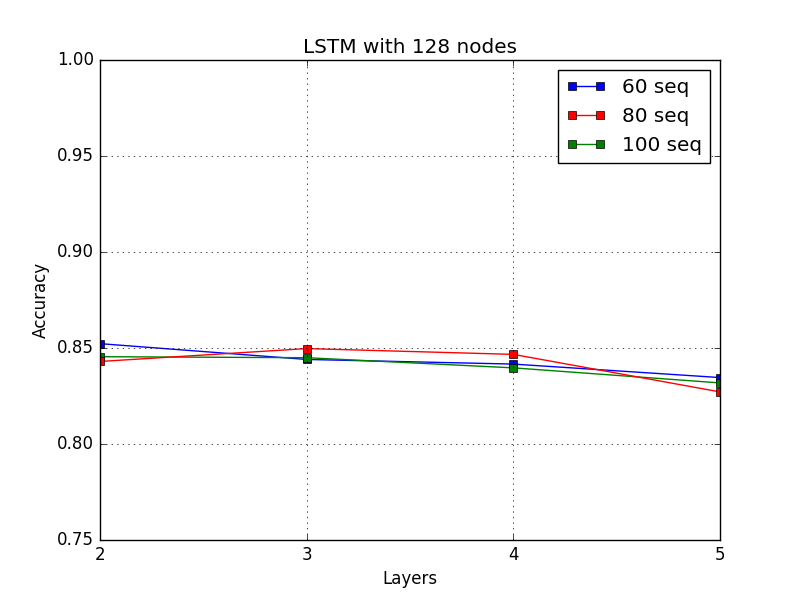
\includegraphics[width=0.7\textwidth]{./images/plots/english/accuracy_128n_word_min_loss.png}
  \end{center}
  \caption{L'accuratezza di una rete LSTM da 128 nodi, raggruppata per livelli e
          lunghezza di sequenza. Per l'addestramento di questa rete \`e stato
          utilizzato il dataset CoNLL ma non si \`e tenuto conto degli spazi fra
          un token e l'altro}
  \label{fig:accEng128nosp}
\end{figure}

\begin{figure}[H]
  \centering
  \begin{center}
    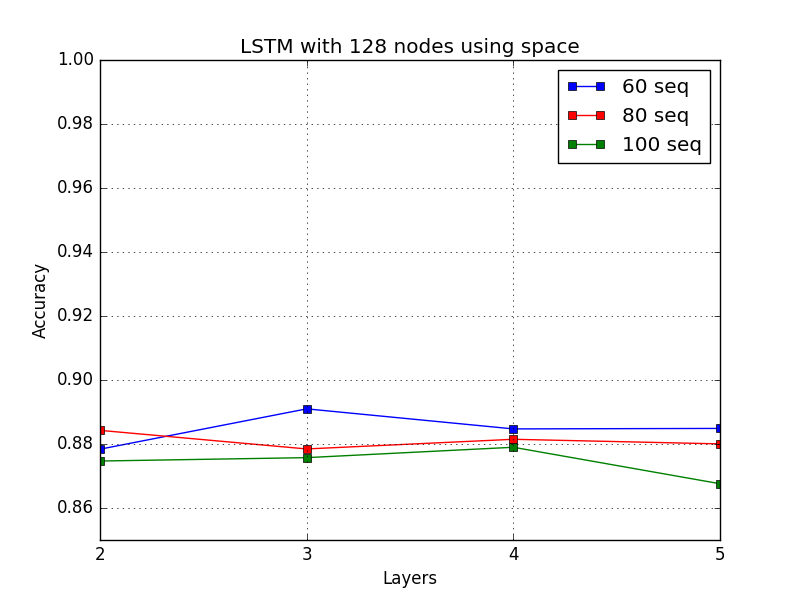
\includegraphics[width=0.7\textwidth]{./images/plots/english/accuracy_128n_word_min_loss_using_spaces.png}
  \end{center}
  \caption{L'accuratezza di una rete LSTM da 128 nodi, raggruppata per livelli e
          lunghezza di sequenza. Per l'addestramento di questa rete \`e stato
          utilizzato il dataset CoNLL e si \`e tenuto conto degli spazi fra un
          token e l'altro}
  \label{fig:accEng128sp}
\end{figure}

Dai grafici \ref{fig:accEng128nosp} e \ref{fig:accEng128sp} risulta evidente che
l'architettura a 128 nodi non offre prestazioni di rilievo, inoltre, la scarsa
varianza data dalla modifica degli altri parametri (livelli e lunghezza di sequenza)
suggerisce che il numero di nodi \`e eccessivamente limitato per riuscire a
gestire adeguatamente la complessit\`a di un PoS-Tagger. Tuttavia questi grafici
sono molto utili per mostrare un fenomeno che \`e costante anche in tutte le altre
reti addestrate. Infatti, le prestazioni delle reti addestrate senza l'uso dello
spazio risultano essere sempre inferiore rispetto alle stesse configurazioni
addestrate, per\`o, introducendo un carattere di spazio fra un token e l'altro.

Altro aspetto notabile \`e che con l'aumentare del numero di nodi migliorano,
mediamente, anche le prestazioni delle reti (figure~\ref{fig:accEng256sp},
 ~\ref{fig:accEng512sp} e ~\ref{fig:accEng1024sp}).

\begin{figure}[H]
  \centering
  \begin{center}
    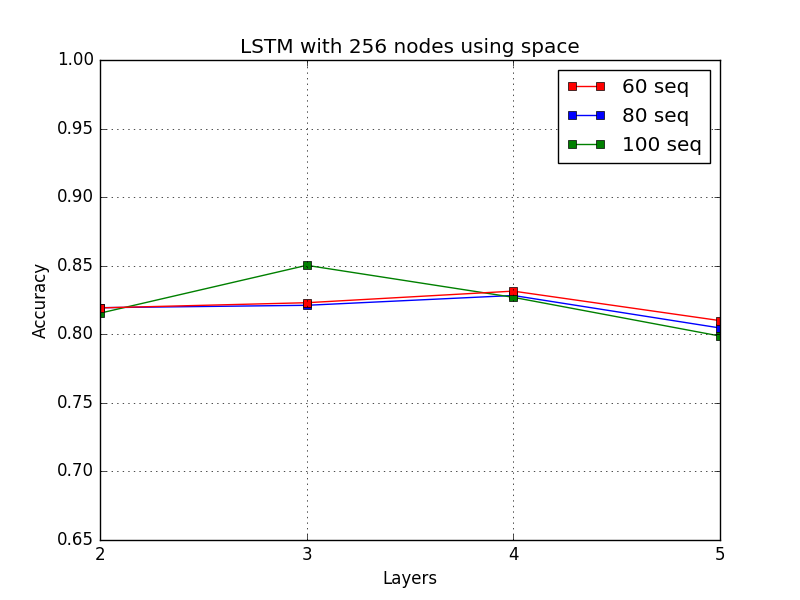
\includegraphics[width=0.7\textwidth]{./images/plots/english/accuracy_256n_word_min_loss_using_spaces.png}
  \end{center}
  \caption{L'accuratezza di una rete LSTM da 256 nodi, raggruppata per livelli e
          lunghezza di sequenza. Per l'addestramento di questa rete \`e stato
          utilizzato il dataset CoNLL e si \`e tenuto conto degli spazi fra un
          token e l'altro}
  \label{fig:accEng256sp}
\end{figure}

\begin{figure}[H]
  \centering
  \begin{center}
    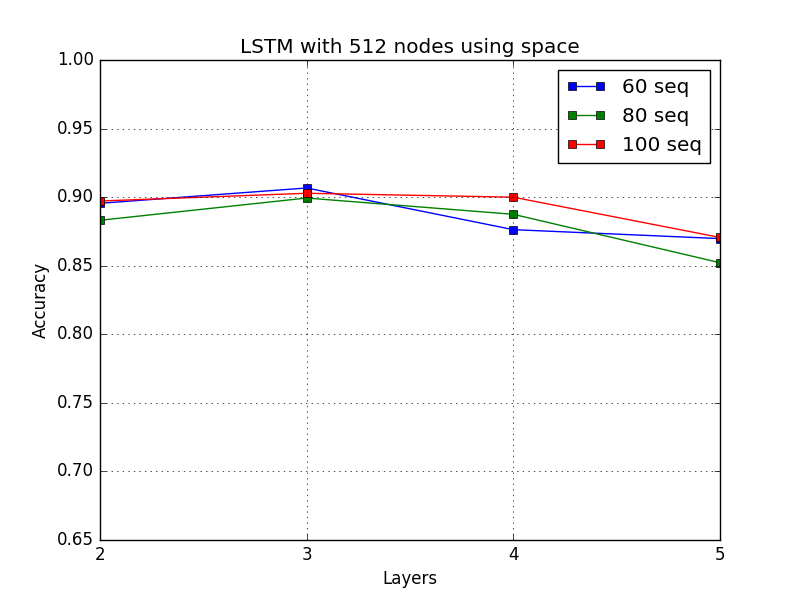
\includegraphics[width=0.7\textwidth]{./images/plots/english/accuracy_512n_word_min_loss_using_spaces.png}
  \end{center}
  \caption{L'accuratezza di una rete LSTM da 512 nodi, raggruppata per livelli e
          lunghezza di sequenza. Per l'addestramento di questa rete \`e stato
          utilizzato il dataset CoNLL e si \`e tenuto conto degli spazi fra un
          token e l'altro}
  \label{fig:accEng512sp}
\end{figure}

\begin{figure}[H]
  \centering
  \begin{center}
    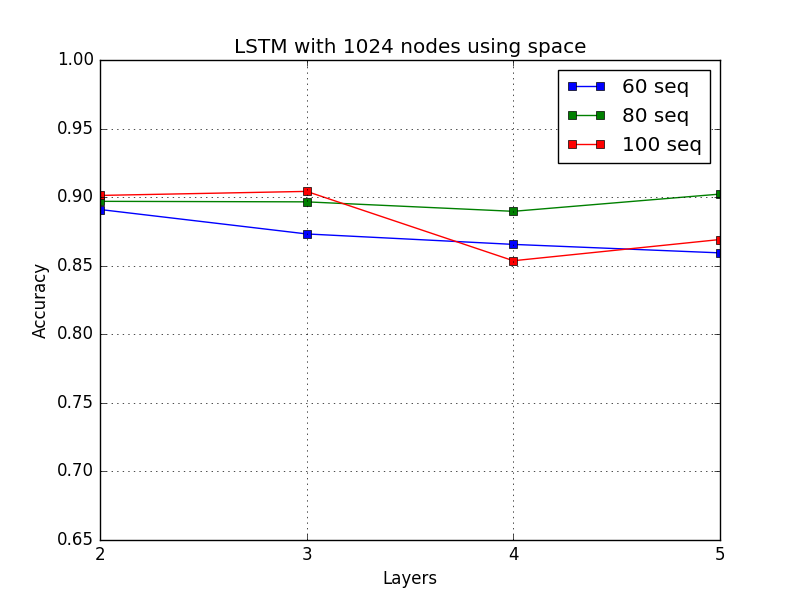
\includegraphics[width=0.7\textwidth]{./images/plots/english/accuracy_1024n_word_min_loss_using_spaces.png}
  \end{center}
  \caption{L'accuratezza di una rete LSTM da 1024 nodi, raggruppata per livelli e
          lunghezza di sequenza. Per l'addestramento di questa rete \`e stato
          utilizzato il dataset CoNLL e si \`e tenuto conto degli spazi fra un
          token e l'altro}
  \label{fig:accEng1024sp}
\end{figure}

Con queste due configurazioni, infatti, si raggiunge anche l'85\% di accuratezza
sul dataset CoNLL2000. Valutare l'impatto che hanno avuto gli altri parametri
nell'apprendimento \`e, tuttavia, pi\`u difficile.

Si pu\`o notare come, nelle configurazioni da 128 e 256 nodi, il numero di livelli
e la lunghezza di sequenza non abbia praticamente alcun impatto di rilievo nelle
performance, mentre nella configurazione da 1024 nodi la lunghezza di sequenza
sembra avere un minimo impatto. Ma si tratta sempre di valori molto piccoli.

Per quanto riguarda la lunghezza di sequenza, il motivo per cui non ha avuto un
grosso impatto nelle performance generali, si pu\`o ricercare nel fatto che
difficilmente le frasi del dataset sono pi\`u lunghe di 60 caratteri. Questo si
traduce nel fatto che la classe assegnata all'ennesimo carattere della sequenza,
non sar\`a influenzato dai 60 o pi\`u caratteri che l'hanno preceduto nella
sequenza. Quindi, aumentare questo valore, non porta a reali benefici.

Tuttavia, non so dare una motivazione adeguata alla poca influenza che hanno avuto
i livelli nei risultati ottenuti.

I risultati mostrati fino ad ora sono riferiti al dataset CoNLL che, ricordiamo,
\`e taggato con un tagset che conta, circa, 40 classi. I risultati ottenuti con
il dataset Evalita presentano le medesime caratteristiche dei risultati precedenti
ma risultano essere mediamente pi\`u bassi. Ad esempio si prendano in considerazione
i grafici \ref{fig:accEva512sp} e \ref{fig:accEva1024sp}:

\begin{figure}[H]
  \centering
  \begin{center}
    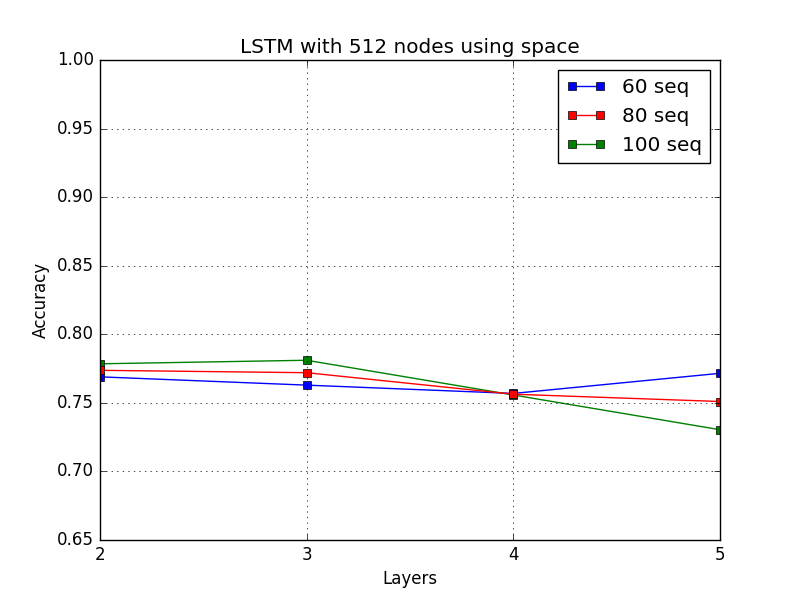
\includegraphics[width=0.7\textwidth]{./images/plots/evalita/accuracy_512n_word_min_loss_using_spaces.png}
  \end{center}
  \caption{L'accuratezza di una rete LSTM da 512 nodi, raggruppata per livelli e
          lunghezza di sequenza. Per l'addestramento di questa rete \`e stato
          utilizzato il dataset Evalita e si \`e tenuto conto degli spazi fra un
          token e l'altro}
  \label{fig:accEva512sp}
\end{figure}

\begin{figure}[H]
  \centering
  \begin{center}
    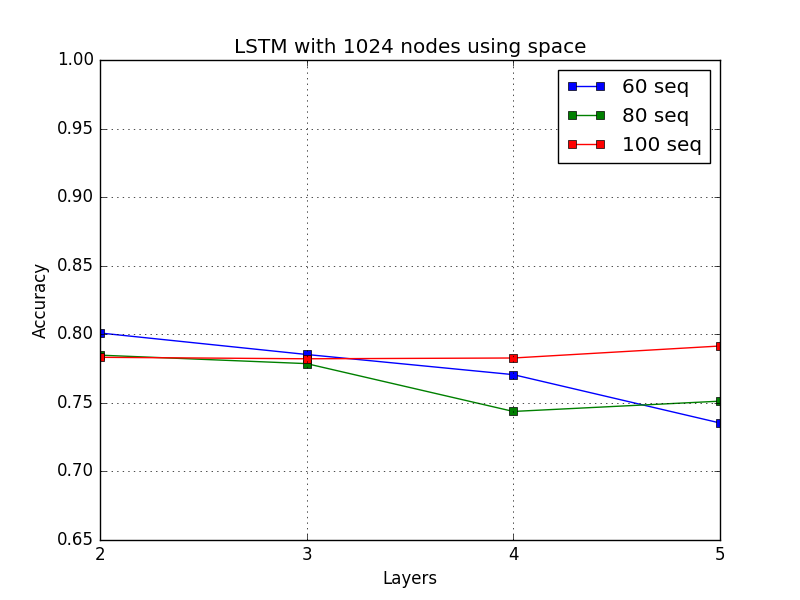
\includegraphics[width=0.7\textwidth]{./images/plots/evalita/accuracy_1024n_word_min_loss_using_spaces.png}
  \end{center}
  \caption{L'accuratezza di una rete LSTM da 1024 nodi, raggruppata per livelli e
          lunghezza di sequenza. Per l'addestramento di questa rete \`e stato
          utilizzato il dataset Evalita e si \`e tenuto conto degli spazi fra un
          token e l'altro}
  \label{fig:accEva1024sp}
\end{figure}


Questi risultati, sostanzialmente pi\`u bassi rispetto a quelli ottenuti con CoNLL,
sono di certo motivati dal fatto che il dataset Evalita \`e stato taggato usando
un tagset con pi\`u di 300 classi. Questo, unito alle modeste dimensioni del dataset
usato per l'addestramento, hanno sicuramente portato a risultati in generale pi\`u
bassi.



% ----------------------------------------------------------------

\bibliographystyle{plain} %mettere plain o alpha
\bibliography{bibliography}

% ----------------- Insert index
%\addcontentsline{toc}{chapter}{Index of terms}
%\printindex
%\input{tesi.ind}
\clearpage
\vspace*{6cm}

% ----------------------------------------------------------------
\end{document}
% ----------------------------------------------------------------
